%==============================================================================    
\chapter{Pixel chip electronics and calibration}
\label{ch:FE_electronics}
%==============================================================================    

% ----------------------------- %
\tikzstyle{block} = [rectangle, draw, text width=5em, text centered, rounded corners, minimum
height=4em]
\usetikzlibrary{backgrounds,fit,decorations.pathreplacing} 
% ----------------------------- %

One of the key components of the detector systems is the readout
electronics. Each experiment, depending on the requirements, has its
own specific electronics. But the basic principles of the electronics
and optimisations of the signal-to-noise remain similar between
different applications.

In this chapter, we will review the basic principles and requirements
of the Timepix3 hybrid pixel readout chip which are used to study thin
and active-edge sensors as described in the following chapters. The
calibration method for the Timepix3 ASICs and also the noise
measurements are explored in this chapter.

%\section{Generic pixel chip properties}
\section{The Timepix3 hybrid readout ASICs}
\label{sec:TimepixChip}

The hybrid readout chip acquires the short ionisation current pulses
generated in the sensor by the passing of a high energetic
particle. The electronics are responsible for shaping the time
response of the system in order to optimise the minimum detectable
signal, energy deposition in detector measurement, event rate,
time-of-arrival and insensitivity to the pulse shape. Finally, the
signal is digitised and stored. Robustness to radiation and low power
consumption are other important considerations to be addressed amongst
others.


%% Timepix3 description
%% \section{The Timepix readout chip families}\label{sec:TimepixReadout}
The Timepix~\cite{art:tmpx,Timepix3Poikela} hybrid pixel detector
readout chip family, designed by the Medipix collaboration, is a
general purpose front-end electronics and can measure precisely the
energy deposited in the sensor and also provides accurate timing
information. This chip is used in a wide range of applications such as
high energy physics and medical imaging. The Timepix3 ASICs are
deployed for the CLIC vertex detector R\&D to study the feasibility of
thin sensors and also active-edge sensors as described in the coming
chapters. 

\cref{fig:detectorFunctions} schematically shows the basic signal flow
in a Timepix3-like hybrid pixel detector. Both analogue and
digital circuitry are combined. 

The incident radiation deposits energy in the sensor and it is
converted to an electrical signal. A high rate of particles can be
handled in a semiconductor detector because the sensor pulse is very
short (few nanoseconds). Since the magnitude of the signal charge is
small and subject to statistical fluctuations (\cref{sec:chargeInSi}),
a charge sensitive preamplifier is needed to amplify the signal. The
preamplifier should be designed in such a way to minimise the
electronic noise. The sensor capacitance and the input capacitance of
the amplifier are the critical parameters to increase the
signal-to-noise ratio (SNR): the lower the capacitance, the higher the
SNR. The amplification is done with a tunable discharge current of the
Krummenacher amplifier architecture
(I\textsubscript{krum})~\cite{KRUMMENACHER1991527}.

After the preamplifier, the pulse shaper is responsible for the
improvement of the SNR. It modifies the frequency response of the
signal to improve the signal and attenuate the noise. Since this
operation reduces the bandwidth of the signal, the duration of the
pulse will increase. A detector must cope with a high rate of pulses,
the width of the pulse must be optimised in a way to reduce the
pile-up. I\textsubscript{krum} affects the slope of the pulse
discharge after shaping: the higher its value, the shorter the
pulse.

The discriminator is used to compare the signal level to a
threshold (a voltage) and to discriminate a signal from a background
noise. Both polarities (electrons and holes collection) are accepted
by the front end.

The analog-to-digital converter (ADC) converts a continuously varying
amplitude to discrete steps. When the pulse height passes a threshold
in a comparator, counters are incremented to measure the energy and
the timing of the signal for example.

\begin{figure}[htbp]
  \centering
  \begin{tikzpicture}[node distance = 2.5cm, auto]
    \begin{scope}[x={(image.south east)},y={(image.north west)}]

      \coordinate (input);
      \node [block, right of=input] (sens) {Sensor};
      \node [block, right of=sens] (preamp) {Preamplifier};
      \node [block, right of=preamp] (pulse) {Pulse shaping};
      \node [block, right of=pulse] (discr) {Discriminator};
      \node [block, right of=discr] (conv) {ADC converter};
      \coordinate[right of=conv] (output);

      \draw[arrows=->] (input) -- node [text
      width=2cm,midway] {Incident radiation} (sens);
      \draw[arrows=->] (sens) -- (preamp);
      \draw[arrows=->] (preamp) -- (pulse);
      \draw[arrows=->] (pulse) -- (discr);
      \draw[arrows=->] (discr) -- (conv);
      \draw[arrows=->] (conv) -- node [text width=1.5cm,midway]
      {Digital data bus} (output);

      % \draw[] (sens) -- (discr.south);
      \draw[decorate,decoration={brace, mirror}, thick] (sens.south) to
      node[below,below] (bracket) {Analogue}
      (discr.south);

      \draw[decorate,decoration={brace, mirror}, thick] (conv.south west) to
      node[below,below] (bracket) {Digital}
      (conv.south east);

    \end{scope}
  \end{tikzpicture}
  \caption{Schematic overview of basic signal flow in a hybrid pixel
    detector. The energy deposited in the sensor by the incident
    radiation is converted to an electrical signal. The signal is
    integrated in the preamplifier, shaped by the pulse shaper and
    compared to a programmable threshold by the discriminator. The
    analogue-to-digital converter (ADC) digitises the signal for
    storage and analysis.}  
  \label{fig:detectorFunctions}
\end{figure}


An overview on the Timepix3 readout chip is given
in~\cref{tab:timepixOverview}. It consists of a $256\times256$ pixel
matrix with pixels pitch of $55\,\micron$. This chip allows for three
operation modes: photon counting (PC), Time-over-threshold (TOT) and
Time-of-Arrival (TOA) measurements. In addition, Timepix3 allows for
simultaneous measurement of the TOT and the TOA.

\begin{table}[htbp]
  \centering
  \caption{Overview of the Timepix3 readout ASICs.}
  \label{tab:timepixOverview}
  \begin{tabular}{l c}
    \toprule
    Pixel Matrix& $256\times256$\\
    Pixel Pitch [\micron] & 55\\
    Technology & 130~nm CMOS\\
    Counter Depth & 10 bit TOT and 18
                            bit TOA \\
    Clock speed & up to 40~\megahertz for TOT and 640~\megahertz for
                  TOA \\
    Readout Type & Data driven \& frame based \\
    Electronic Noise without sensor & $<70$ e\textsuperscript{-} RMS\\
    \bottomrule
  \end{tabular}
\end{table}


In the photon counting mode, a counter is incremented each time a
photon hits the pixel and deposits an energy higher than the
programmable threshold.
 
\cref{fig:TOT_TOA_concept} schematically shows the energy and the
timing measurement of the signal. The Time-over-threshold (TOT) allows
for the measurement of the energy deposited in a pixel. The pulse is
amplified and the pulse shaper integrates the signal to form a step
pulse with a long approximately linear decay. The time above the
programmable threshold is proportional to the energy deposited and
during this time, the TOT counter is incremented.

The Time-of-Arrival (TOA) measures the arrival time of a hit and
therefore is used as a time stamping of the hits. When the amplifier
output exceeds the pixel threshold, the discriminator output rises and
the fast TOA (FTOA) counter counts until the rising edge of the
general clock. A combination of the TOA and the FTOA counters is used
as the timing information for the hits.

\begin{figure}[htbp]
  \centering
  \begin{tikzpicture}
    \begin{scope}[x={(image.south east)},y={(image.north west)}]
      % pulse
      \draw[-, thick] (0.1, 0.8) -- (0.2, 0.8);
      \draw[-, thick] (0.2, 0.8) -- (0.21, 0.98);
      \draw[-, thick] (0.21, 0.98) -- (0.22, 0.8);
      \draw[-, thick] (0.22, 0.8) -- (1, 0.8);

      % shaper
      \draw[-, thick] (0.1, 0.5) -- (0.2, 0.5);
      \draw[-, thick] (0.2, 0.5) -- (0.22, 0.7);
      \draw[-, thick] (0.22, 0.7) -- (0.8, 0.5);
      \draw[-, thick, dashed, green] (0.1, 0.55) -- (0.8, 0.55);
      \draw[-, thick] (0.8, 0.5) -- (1, 0.5);

      % comparator
      \draw[-, thick] (0.1, 0.3) -- (0.21, 0.3);
      \draw[-, thick] (0.21, 0.3) -- (0.21, 0.4);
      \draw[-, thick] (0.21, 0.4) -- (0.65, 0.4);
      \draw[-, thick] (0.65, 0.4) -- (0.65, 0.3);
      \draw[-, thick] (0.65, 0.3) -- (1, 0.3);

      \timing [] at (0.11, 0.2) {HLLHHLLHHLLHHLLHHLLHHLLHH};
      \draw[arrows=<->, thick](0.21, 0.15)--(0.65, 0.15) node [pos=0.5, below]
      {\textbf{TOT (3 counts)}};

      \timing [] at (0.1,0.0) {llllllhlhlhlhllllllllllllllllllllllllllllllllllllll};

      \draw[-, thick, dashed, blue] (0.21, 0.55) -- (0.21, 0.0);
      \draw[-, thick, dashed, blue] (0.65, 0.55) -- (0.65, 0.0);

      \draw[-, thick, dashed, red] (0.355, 0.2) -- (0.355, 0.0);

      \draw[arrows=<->, thick](0.21, -0.05)--(0.35, -0.05) node [pos=0.5, below]
      {\textbf{FTOA (4 counts)}};


      \node[left] at (0.1, 0.8) {Sensor pulse};
      \node[left, green] at (0.1, 0.6) {Threshold};
      \node[left] at (0.1, 0.5) {Pulse after shaping};
      \node[left] at (0.1, 0.3) {Discriminator output};
      \node[left] at (0.1, 0.2) {General clock}; %$40\,\megahertz$ Clk}
      \node[left] at (0.1, 0.0) {FTOA clock}; %$640\,\megahertz$ Clk (FTOA)     


    \end{scope}
  \end{tikzpicture}
  \caption{Schematic overview of the Time-over-Threshold (TOT) and
    Time-of-Arrival (TOA) measurements for the Timepix3 readout chips.}
  \label{fig:TOT_TOA_concept}
\end{figure}


\subsection{SPIDR readout system for Timepix3}\label{sec:TimepixReadout}

The SPIDR (Speedy PIxel Detector Readout) readout system has been
developed by NIKHEF and CERN is used~\cite{Visser:2015bsa} for the
Timepix3 data acquisition. This system is able to handle high rates of
data sent by the Timepix3 ASIC at full speed. This is achieved with
Xilinx Virtex-7 FPGA~\cite{XilinxVirtex7} and a 10~Gb Ethernet link.

\begin{figure}[htbp] \centering
  \begin{subfigure}[b]{0.3\textwidth}
    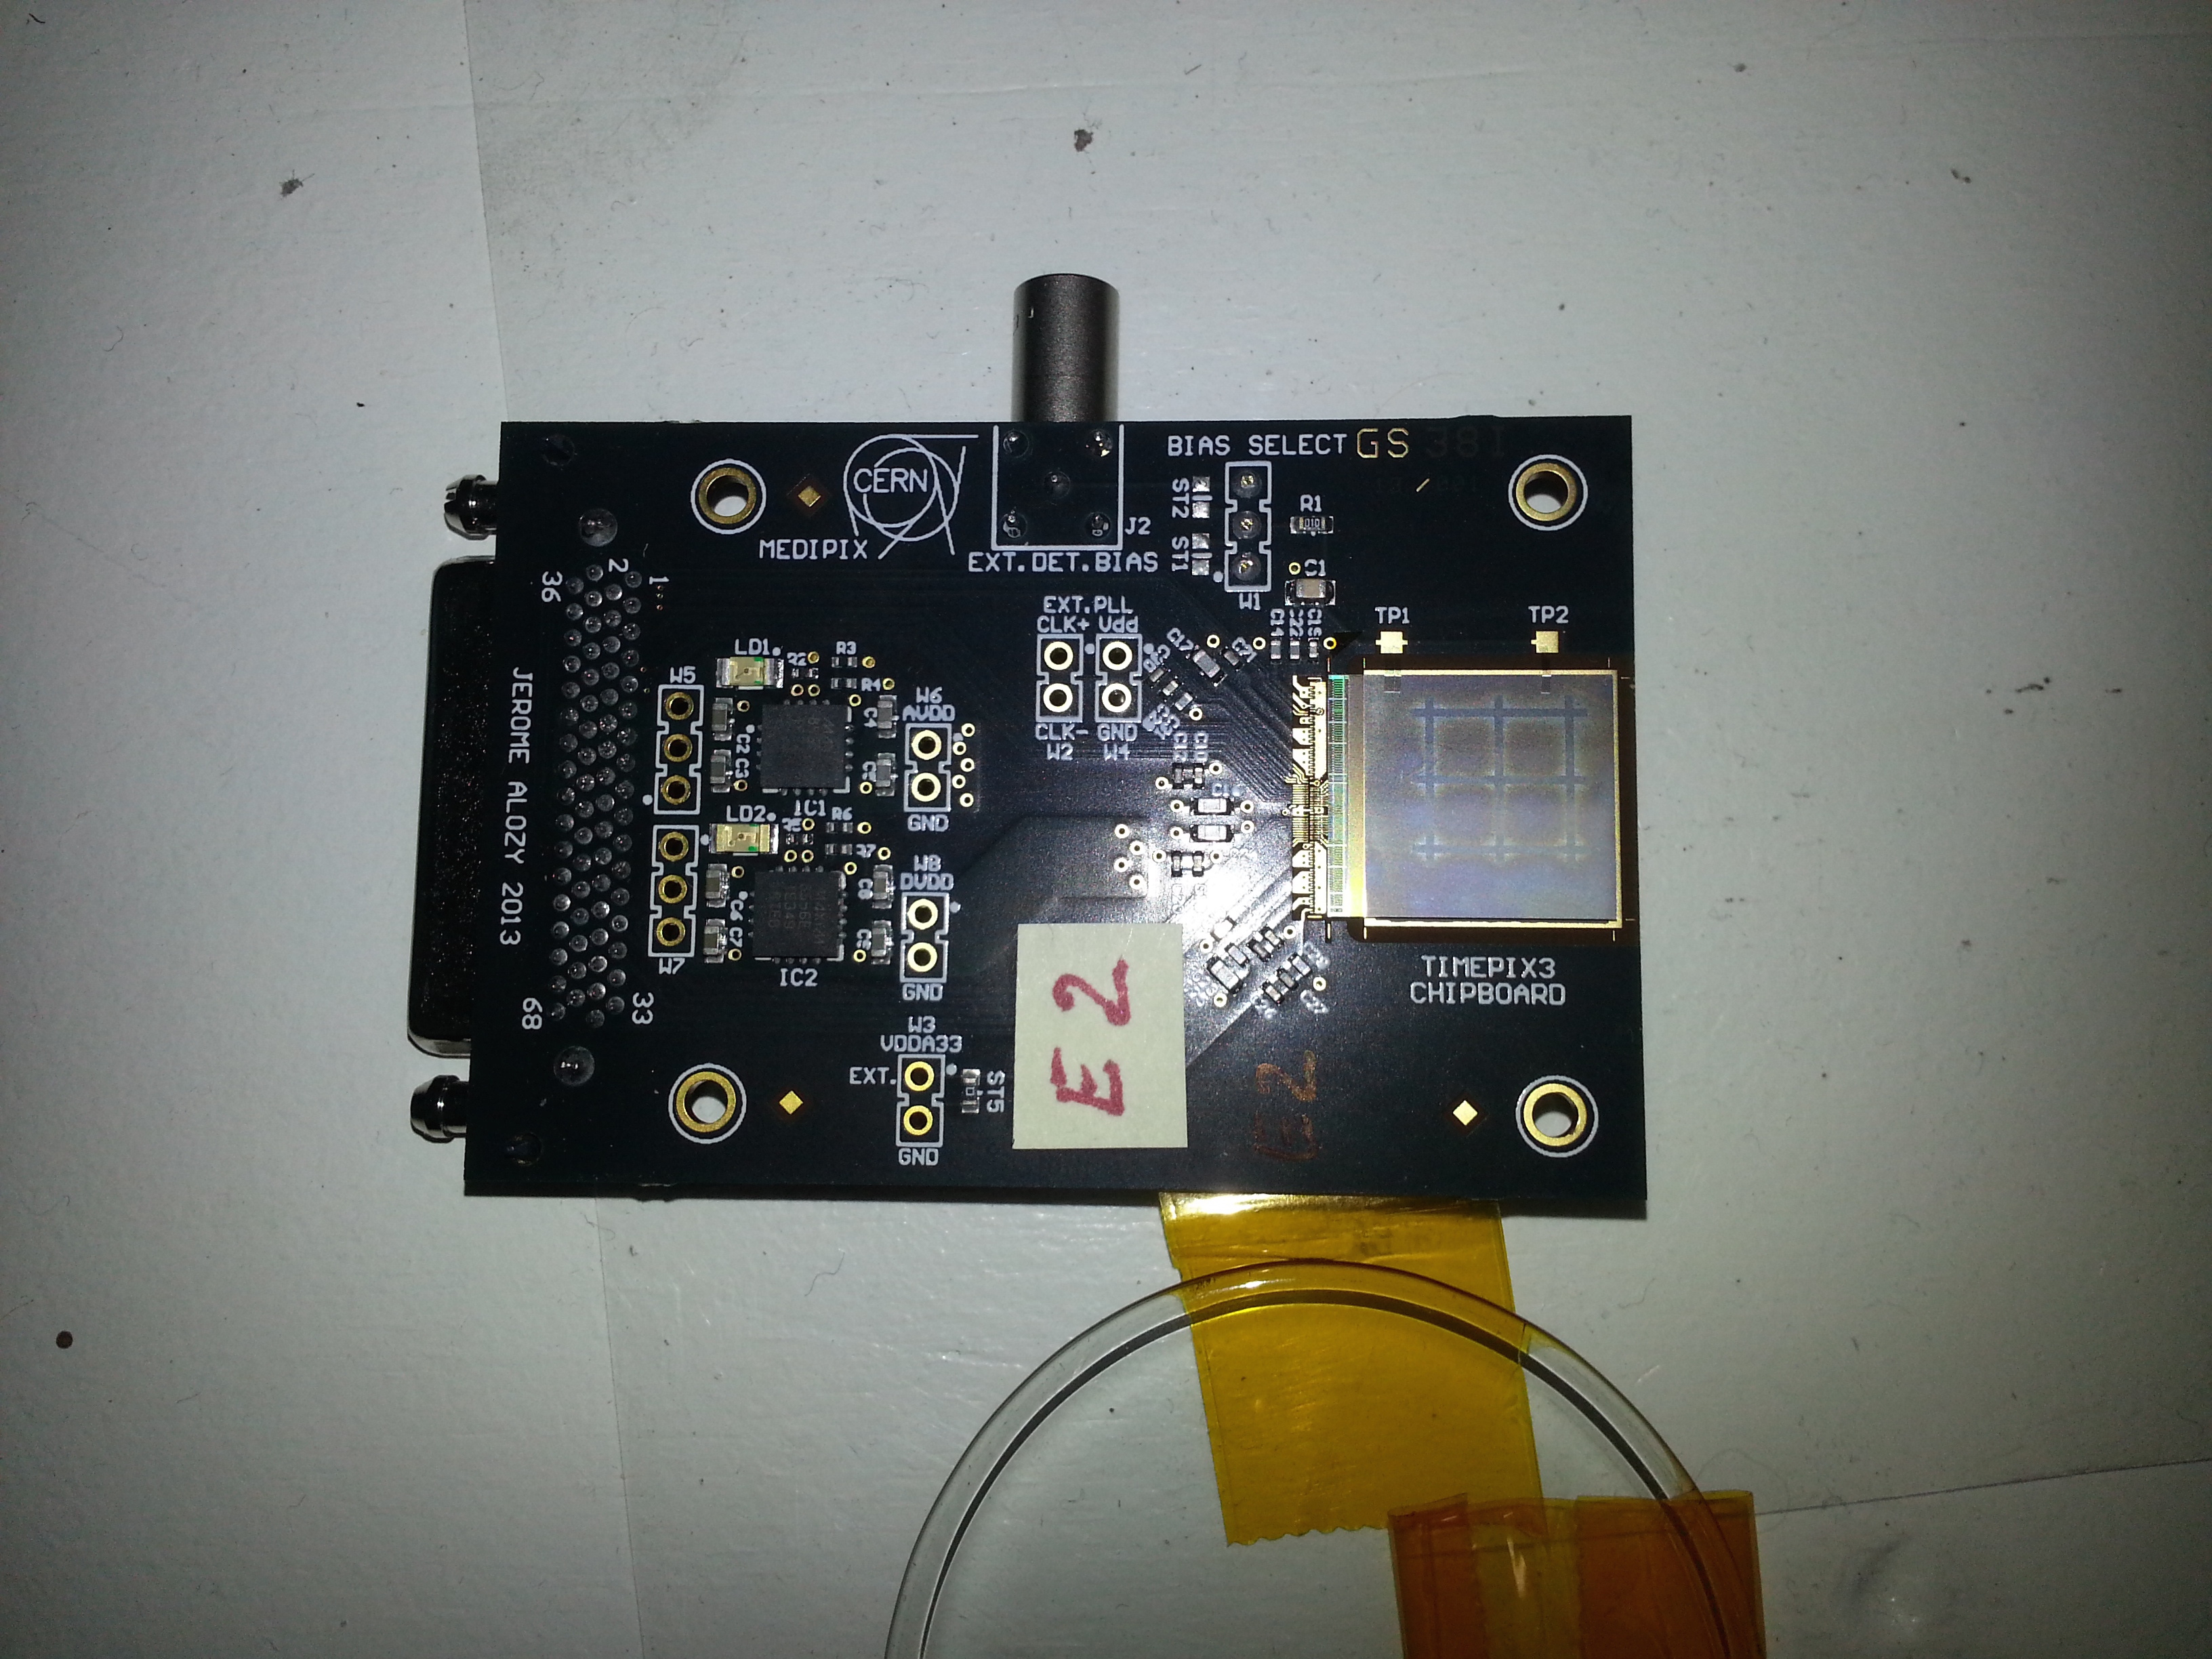
\includegraphics[width=\textwidth]{./figures/Calibration/Timepix3board.jpg}
    \caption{}\label{fig:Timepix3board_PCB}
  \end{subfigure}\hfill
  \begin{subfigure}[b]{0.65\textwidth}
    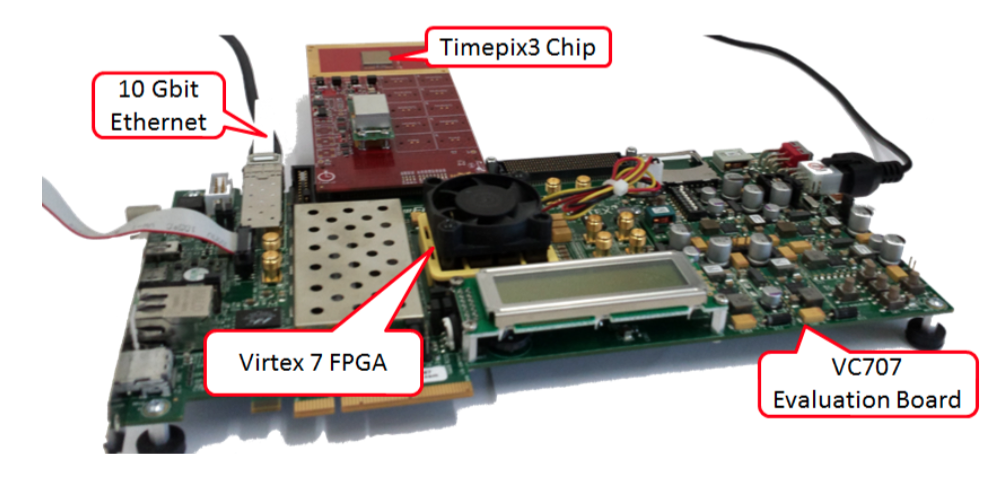
\includegraphics[width=\textwidth]{./figures/Calibration/SPIDRboard.png}
    \caption{}
  \end{subfigure}
  \caption{(a) Timepix3 chip board and (b) SPIDR readout board.}
  \label{fig:Timepix3board_SPIDR}
\end{figure}

The Timepix3 readout chip allows for a data-driven zero-suppressed
readout mode which can reach higher readout rates than the frame based
mode. In the data driven mode, after a hit is processed by the pixel,
a data packet containing the TOT and the TOA information is
immediately sent off the chip. This reduces significantly the dead
time of the pixels and allows to reach very high readout rates of up
to 40~Mhits/s/\cmsquared.

The different settings of the chip are controlled externally using
programmable DACs such as the I\textsubscript{krum}, threshold,
polarity of the sensor and the clock speed.

%% --------------------------------------------- %%
\section{Timepix3 assemblies}\label{sec:Timepix3Assemblies}
A summary of the Timepix3 assemblies is shown in
\cref{tab:Timepix3Assemblies}. Advacam sensors~\cite{AdvacamRef} of
thickness $50$-$300\,\micron$ are bump-bonded to Timepix3 readout
chips.

\begin{table}[htbp]
  \centering
  \caption{Details of different Advacam planar pixel sensors
    bump-bonded to Timepix3 readout ASICs and studied in calibration
    and test beams. For active-edge sensors, the edge distance is
    defined by the distance between the last pixel implant and the
    physical sensor edge.}
  \label{tab:Timepix3Assemblies}
  \resizebox{\textwidth}{!}{\begin{tabular}{lccccc}
    \toprule
    Timepix3 ID & Thickness [\micron] & Type & Edge distance [\micron] & Guard-ring potential & Assembly\\
    \midrule
     W19\_G7 & 50 & n-in-p & 20 & Without GR & 20-NGR-50 \\
     W19\_F7 & 50 & n-in-p & 23 & Floating & 23-FGR-50 \\
     W19\_L8 & 50 & n-in-p & 28 & Grounded & 28-GNDGR-50 \\
     W19\_C7 & 50 & n-in-p & 55 & Grounded & 55-GNDGR-50 \\ \hline
     W5\_E2 & 100 & n-in-p & 55 & Grounded & 55-GNDGR-100 \\ \hline
     W5\_F1 & 150 & n-in-p & 55 & Grounded & 55-GNDGR-150 \\ \hline
     W2\_J5 & 300 & p-in-n & - & - & - \\
    \bottomrule
  \end{tabular}}
\end{table}

%% --------------------------------------------- %%
\section{Electronic noise}\label{sec:noise}

Electronic noise places a limit on the minimum detectable signal
level, defines the ability to distinguish signal levels and their
precision of measurement. Thermal excitations and sensor leakage
currents are important sources for the noise. The electronic noise can
be measured as explained further in
\cref{sec:thresholdCalibration}. For Timepix3 readout chips, the
electronic noise before bonding to any sensor is less than
70~e\textsuperscript{-} RMS and after bonding it increases to
$\sim80$~e\textsuperscript{-} RMS due to the capacitance of the sensor
and its leakage current.

The electronic noise is an important parameter to determine the
operating threshold of the readout chip. In fact, the operating
threshold for the Timepix3 chip is set to 6 times the electronic noise
RMS. This threshold significantly reduces the detection of noisy
hits. Sometimes at this threshold few pixels show a high rate of hits
in absence of incident radiation (hot pixels) and they are manually
masked to be able to operate the chip at the lowest possible
threshold.

The operating threshold affects significantly the spatial resolution
of the device. A lower threshold allows for a higher detection of the
charge sharing. For this reason, it is important to minimise the
electronic noise.

%% --------------------------------------------- %%
\section{Threshold dispersion and equalisation} 
\label{sec:ThresholdEqualisation}


In semiconductor electronics, manufacturing imperfections cause
variations in the performance within the device. The programmable
global threshold of the chip is one of the most affected
parameters. In fact, the global threshold is programmed through a
programmable DAC (Digital-to-Analog) and is translated to the voltage
applied at the discriminator. The signal level is compared to this
voltage. For the same global threshold value, the voltage on the
discriminator can vary highly from one pixel to another. To overcome
this dispersion, a 4-bit local threshold adjustment is applied to each
pixel in order to make a uniform global threshold. The photon counting
mode is then employed. The equalisation consists of adjusting this
local threshold. First it is set to its minimum value (mask 0000). The
global threshold DAC (THL) is scanned and the number of pixels
responding are counted. Then the adjustment bit is set to its maximum
value (mask 1111) and THL is scanned again. For each pixel, the
operation range is thus known. Assuming a linear relationship between
the two points, the adjustment threshold is adjusted in such a way
that the global threshold will remain uniform across the matrix.

\cref{fig:THLequalisation} shows the threshold equalisation for the
assembly W2\_J5. After equalisation the response of the chip becomes
more uniform even though some dispersion remains.

\begin{figure}[htbp] 
  \centering
  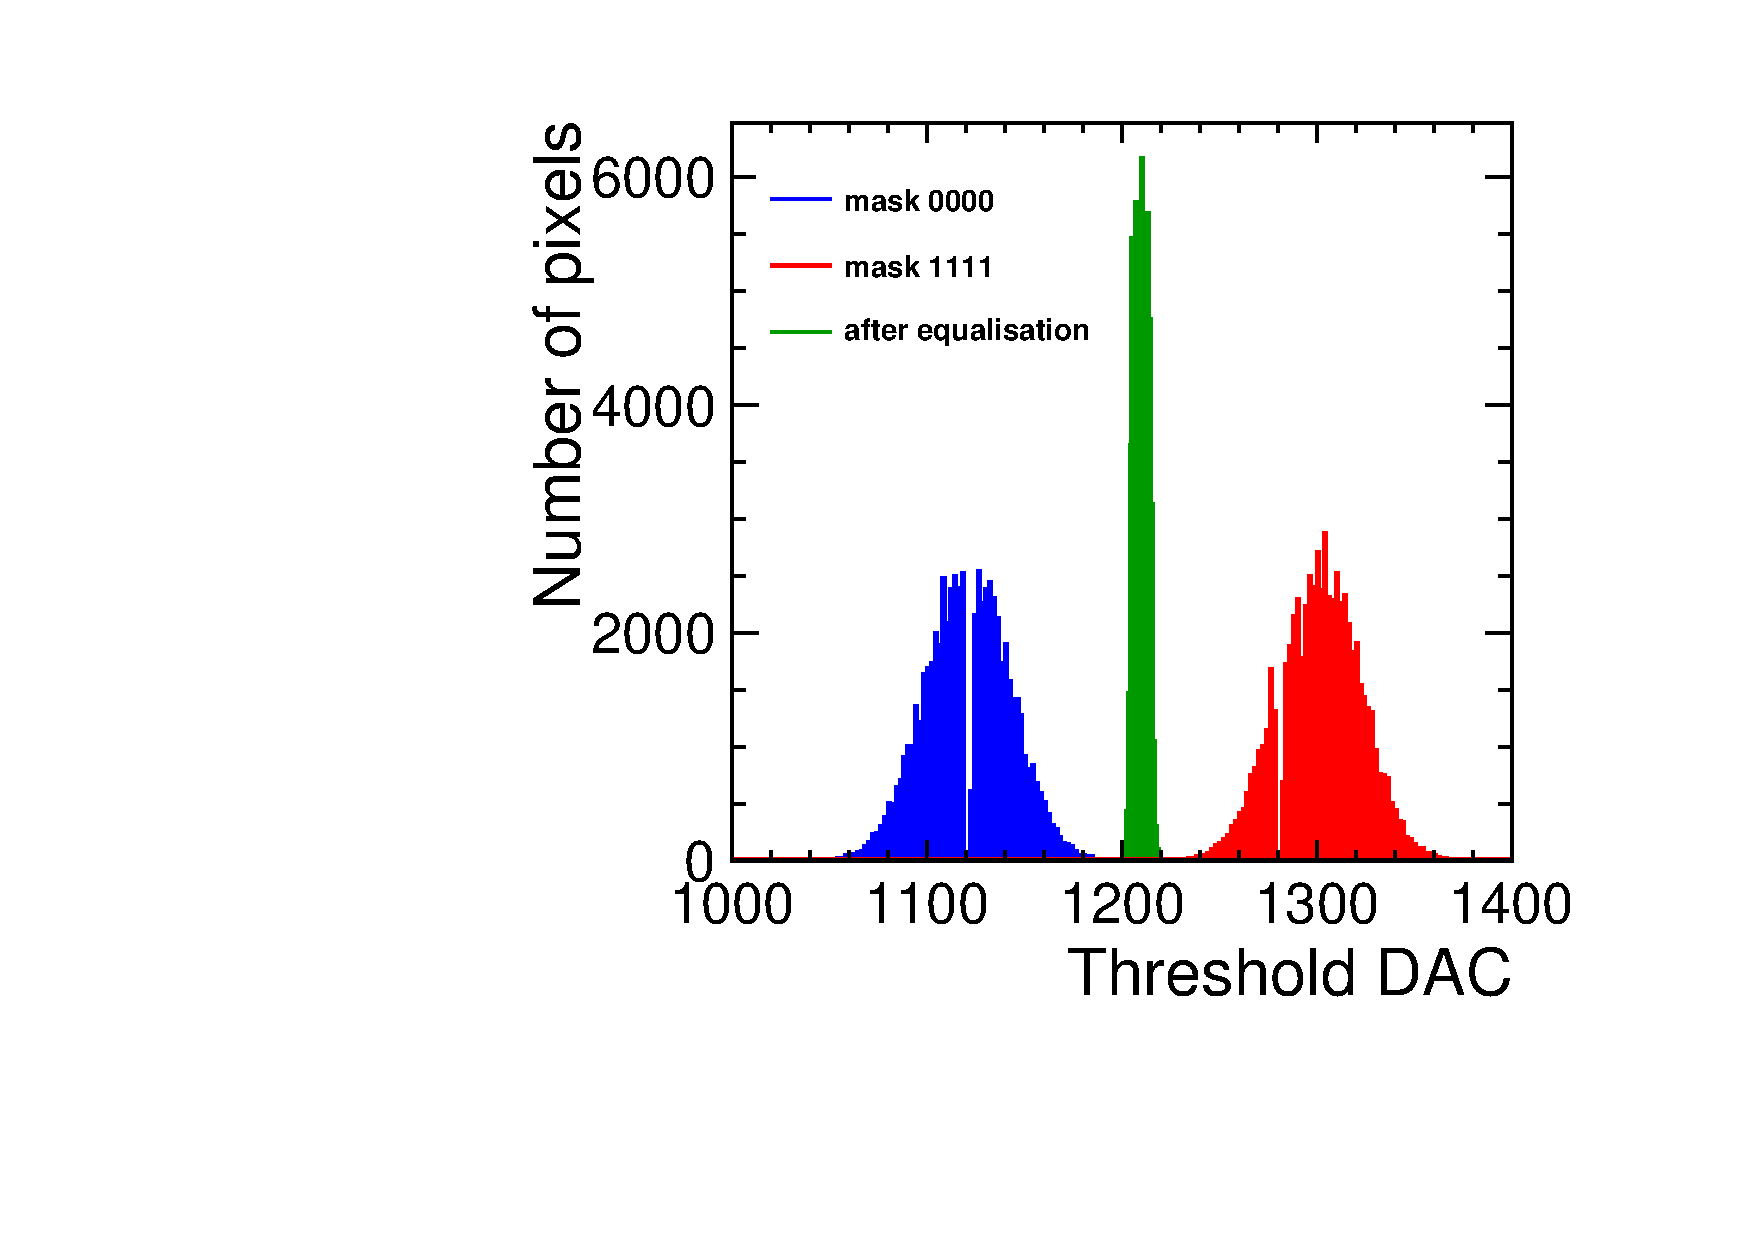
\includegraphics[width=0.6\textwidth]{./figures/Calibration/THLequalisation_W2_J5.pdf}
  \caption{Spread of pixel responses for the assembly W2\_J5 during
    equalisation for the local threshold set at its minimum value
    (mask 0000), to its maximum value (mask 1111) and after
    equalisation.}
  \label{fig:THLequalisation}
\end{figure}

\section{Calibration} \label{sec:calibration} The aim of the
calibration is to parametrise the measurements done by the readout
chip, namely the relationship between the threshold DAC and the TOT
with the energy deposited in the sensor (in number of collected
charge) as well as the relation between the TOA measurement and the
time of arrival of the particle (in seconds). In this work we focus on
the threshold DAC and the TOT calibration.

The threshold DAC and TOT calibration can be achieved using two main
methods. The first one consists of the use of photons from radioactive
sources with a characteristic decay energy or photons from X-ray
fluorescence (XRF) with a characteristic emission
energy~\cite{AlipourTehrani:2054922}. The photon being stopped in the
sensor, it deposits its full energy. Since the energy of the photon is
known, its relation to the threshold DAC or TOT can be characterised. 

The second method consists of the use of an internal analog test pulse
generator. The Timepix3 readout ASICs provide an internal test pulse
generator which can be used for calibration as well as equalisation of
the readout chip. In each pixel, a capacitor allows for injecting a
charge by switching a voltage over it. The charge injected is given by

\begin{equation}
  Q = C \cdot \Delta V \; ,
  \label{eq:testpulseCharge}
\end{equation}

where Q is the injected charge, C the injection capacitance and
$\Delta V$ the voltage applied. A priori, the injection capacitance is
unknown and its value varies from pixel to pixel, but its value can be
measured. For the capacitance, $20.2$~e\textsuperscript{-}/mV is a
good approximation.

In \cref{fig:detectorFunctions}, the injection capacitance replaces
the sensor. For the calibration if the chip is bump-bonded to a
sensor, the sensor is fully depleted with a bias voltage.

\subsection{TOT-energy calibration} \label{sec:EnergyCalibration}

The TOT calibration parametrises the relationship between the energy
deposited (in number of electrons) and the TOT measurement. Due to the
non-linearity of the Timepix3 charge preamplifier, this relationship
is modeled as a hyperbola. The function used to fit the data points is
called a \textit{surrogate function} and is defined as:

\begin{equation}
  \text{TOT} = a \, E + b - \frac{c}{E - t} \; ,
  \label{eq:TOTsurrogateFunction}
\end{equation}

where TOT denotes Time-Over-Threshold, $E$ the energy and $a, b, c, t$
are the parameters to be found~\cite{Jakubek2008155}. The inverse of
the surrogate function is defined as:

\begin{equation}
  E = { {t \cdot a - \text{TOT} -b + \sqrt{\left(b+t \cdot a -\text{TOT}\right)^2+4\cdot a \cdot c}} \over {2a} } \; ,
  \label{eq:inverseTOTsurrogateFunction}
\end{equation}

In \cref{eq:TOTsurrogateFunction}, for higher values of the energy,
the relationship between TOT and $E$ is linear with gradient $a$ and
intercept $b$ since the term $aE+b$ dominates. At low energy, the term
$c/(E-t)$ becomes important. The parameter $c$ defines the amount of
curvature in the function. An asymptote occurs at $E=t$. The point at
which the fit crosses the x-axis (TOT=0) corresponds to the threshold:
below the threshold no charge can be detected. The range for the TOT
and the boundary between low energy (non-linear response) and high
energy (linear response) depend on the clock frequency, the threshold
and the I\textsubscript{krum} value.

For the calibration of the assemblies, the Timepix3 ASICs is operated
in the TOT mode and the test-pulse injection is used
(\cref{eq:testpulseCharge}). Test pulses with heights ranging from
$0\,\mv$ to $800\,\mv$ (corresponding to 0 electrons to 14000
electrons) are sent to each pixel. For each pulse height, 100
test-pulses are sent. The sum of the TOTs and also the sum of the
squared of the TOTs for each pulse height is recorded. The mean of the
TOT response and the standard deviations are then calculated. Finally,
the data are fitted with the surrogate function as given in
\cref{eq:TOTsurrogateFunction} for each pixel and the pixel-by-pixel
energy calibration of the assembly is determined.

\cref{tab:timepix3Operation} summarises the DAC settings used for the
operation of the Timepix3 assemblies in test beams. The same settings
are as well used for the calibration. \cref{fig:TOTcalib_55GNDGR100}
shows the pixel-by-pixel calibration for assembly W5\_E2 operated at
two different threshold DACs of 1160 and 1190. For a higher threshold,
the curves are shifted towards higher energy values on the x-axis but
the slope (parameter $a$) remains the same.

\begin{table}[htbp]
  \centering
  \caption{DAC settings for the operation and calibration of the
    Timepix3 assemblies. VFBK is a programmable DAC to determine the
    baseline voltage of the chip.}
  \label{tab:timepix3Operation}
  \begin{tabular}{ c c c c }
    \toprule
    I\textsubscript{krum} & TOT/TOA Clock & FTOA Clock & VFBK \\
    \midrule
    10 & $40\,\megahertz$ & $640\,\megahertz$ & 150 \\
    \bottomrule
  \end{tabular}
\end{table}

\begin{figure}[htbp] \centering
  \begin{subfigure}[b]{0.45\textwidth}
    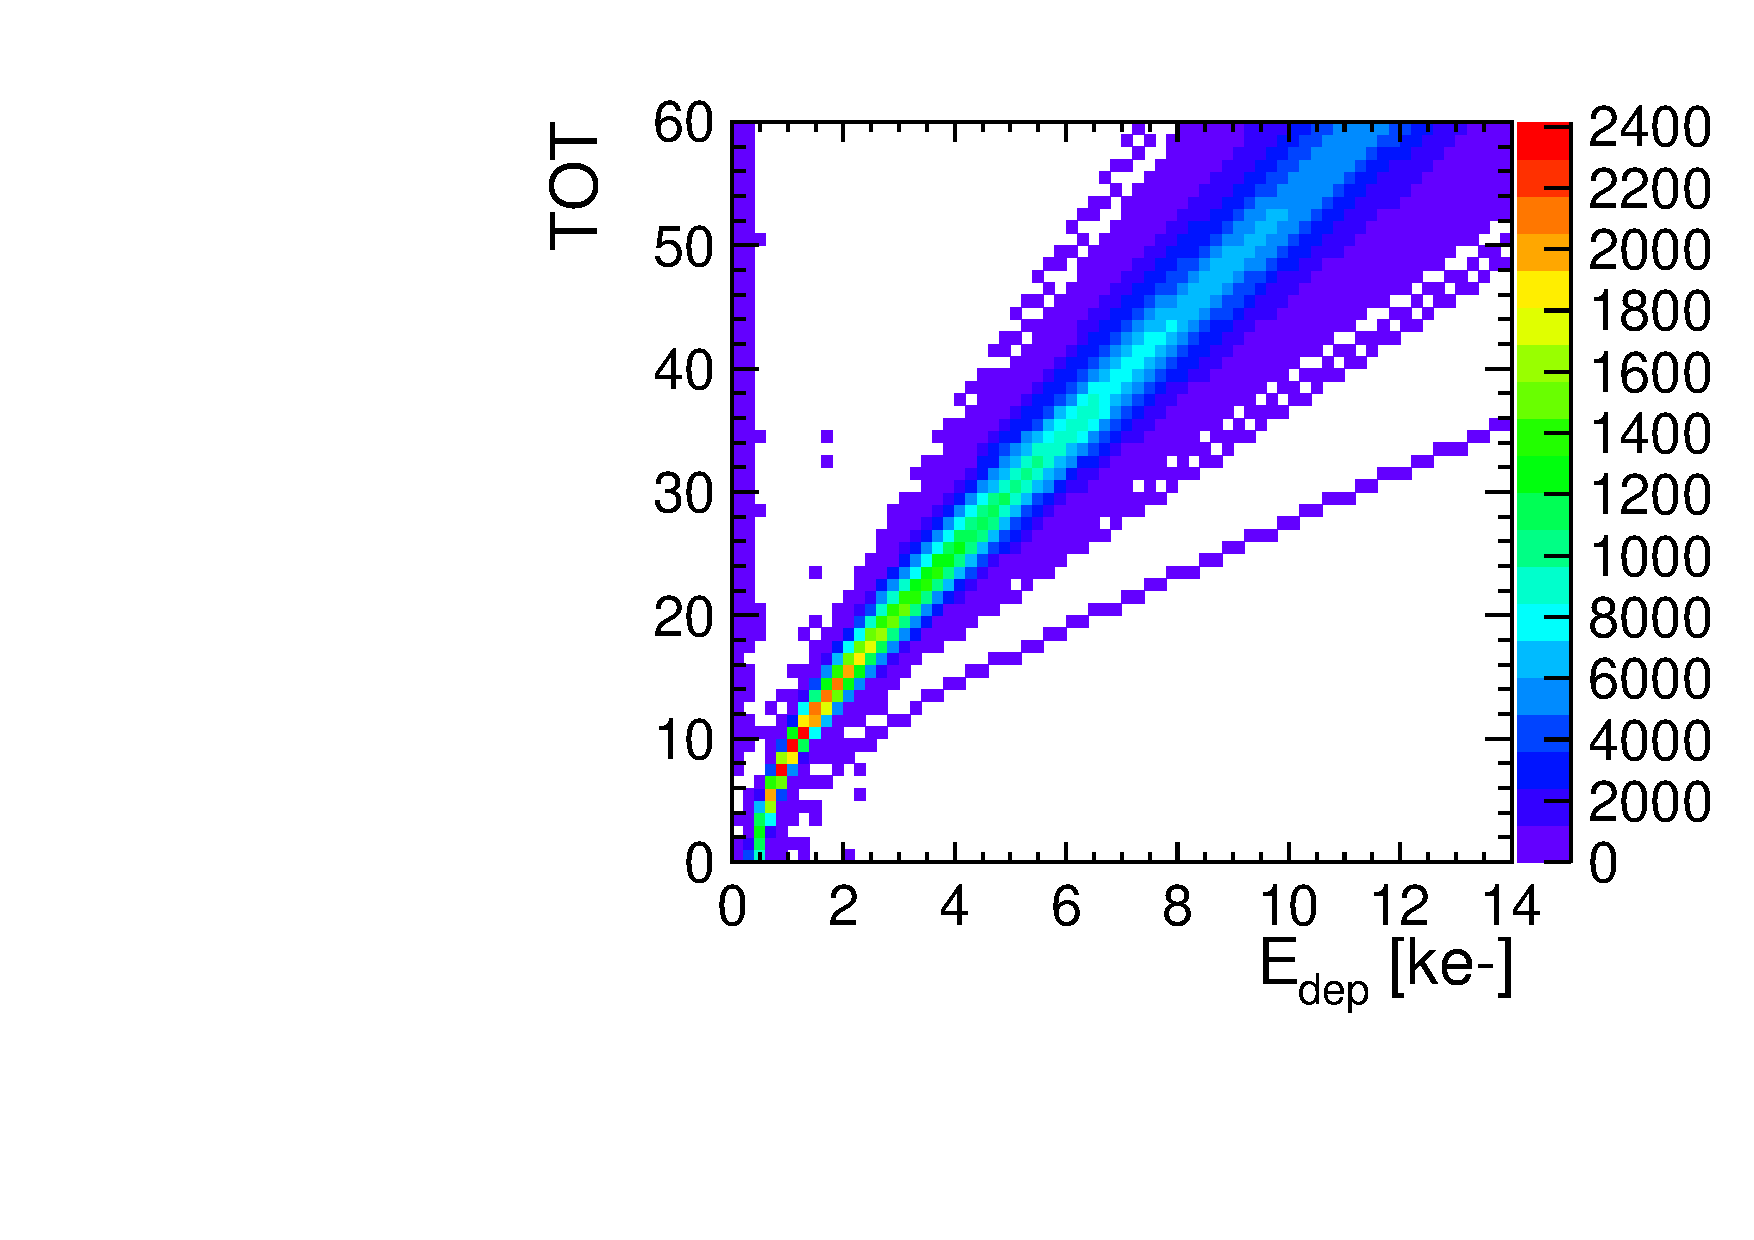
\includegraphics[width=\textwidth]{./figures/Calibration/TOTcalibration_W0005_E02_thresh1160.pdf}
    \caption{}
  \end{subfigure} \hfill
  \begin{subfigure}[b]{0.45\textwidth}
    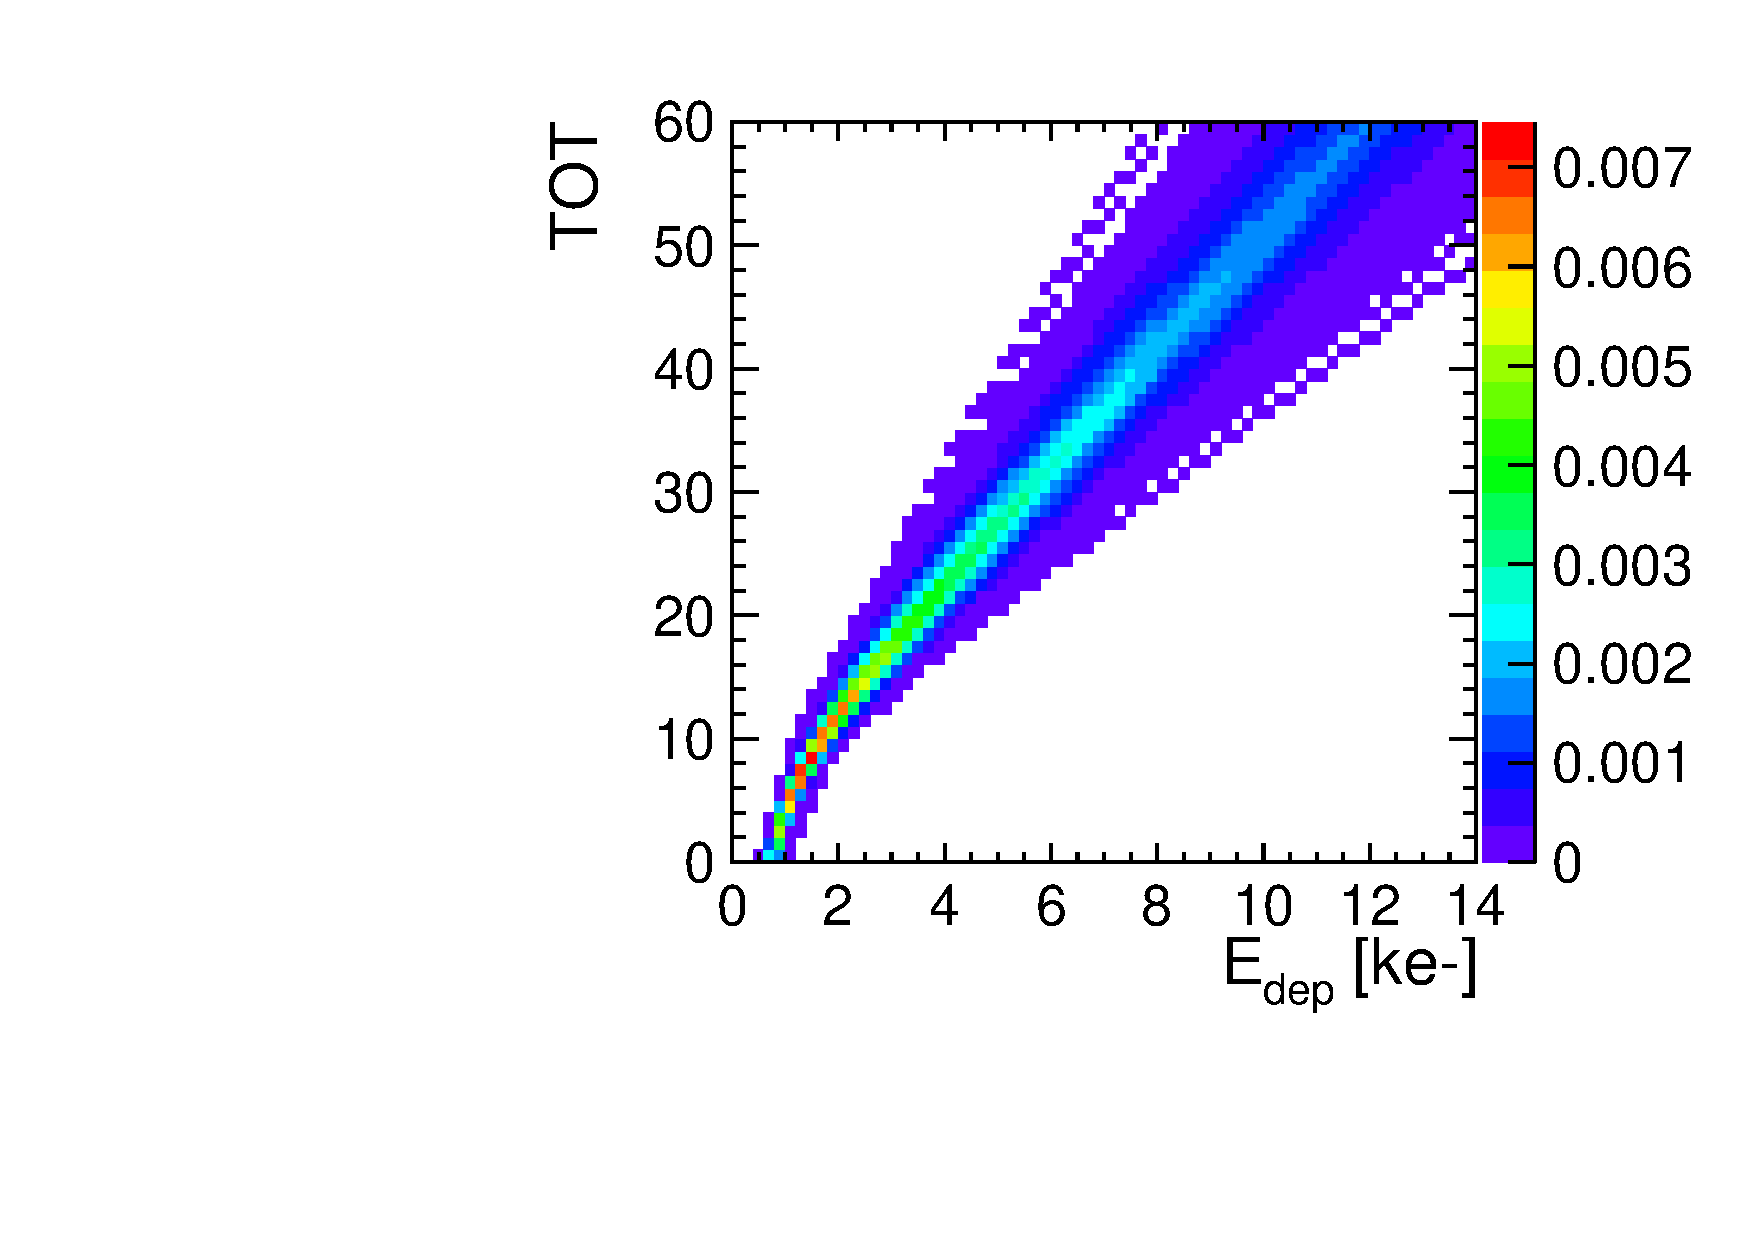
\includegraphics[width=\textwidth]{./figures/Calibration/TOTcalibration_W0005_E02_thresh1190.pdf}
    \caption{}
  \end{subfigure}
  \caption{Pixel-by-pixel calibration of the TOT for assembly W5\_E2
    operated at the threshold DACs of (a) THL=1160 and (b) THL=1190.}
  \label{fig:TOTcalib_55GNDGR100}
\end{figure}

The calibration for the other assemblies are given in
\cref{sec:appendixFE_electronics}.


\subsection{Threshold-energy calibration} 
\label{sec:thresholdCalibration}

\cref{sec:noise} describes the selection of the operating threshold
DAC (Digital-to-Analog Converter) for a Timepix3 readout chip. This
threshold can be translated into an effective energy and used as a
data point for the surrogate fit at the crossing-point on the
$x$-axis. The counting mode is used for this measurement.

For Timepix3 assemblies, the threshold is calibrated using test pulses
at four different heights corresponding to 0, 1000, 3000 and 6000
electrons. For each pulse height, 200 pulses are sent to the pixels in
the diagonal of the matrix and the threshold DAC is scanned with a
step of 2 from a level of no counts (threshold above the signal) to a
level where all the pixels count (threshold close to the noise level)
resulting in an S-shaped curve as shown in
\cref{fig:scurve_example}. The readout electronics noise smears the
ideal sharp turn on and generates the S-curve. At the maximum gradient
of the S-curve, the threshold DAC corresponds to the pulse
amplitude. The derivative of the S-curve is a Gaussian as shown in
\cref{fig:deriv_example} with a mean at the maximum gradient of the
S-curve. The derivative at each point of the S-curve corresponds to
the slope of the line connecting it to its neighbour.

\begin{figure}[htbp] \centering
  \begin{subfigure}[b]{0.45\textwidth}
    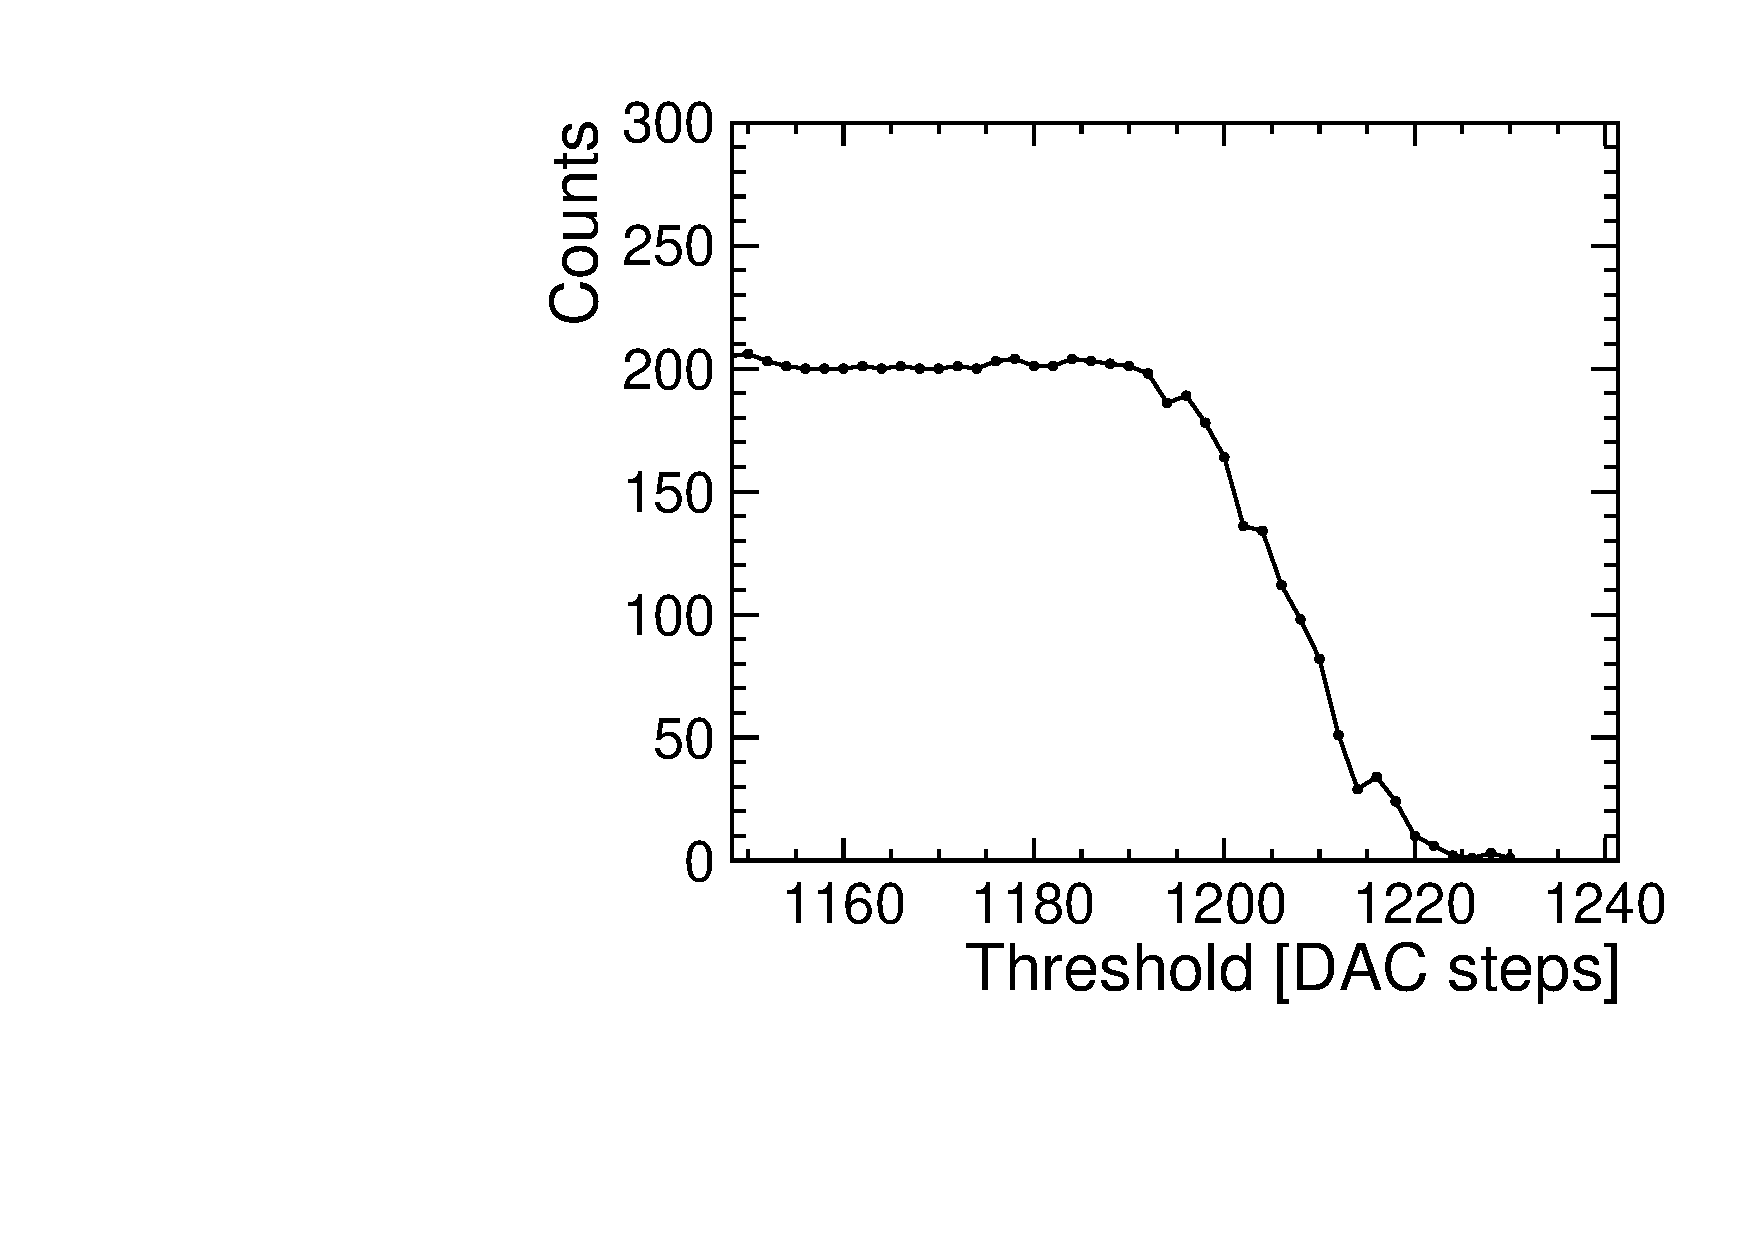
\includegraphics[width=\textwidth]{./figures/Calibration/W5_E2_scurve_ampl1.pdf}
    % \begin{tikzpicture} \node[anchor=south west,inner sep=0] (image)
    %   at
    %   (0,0){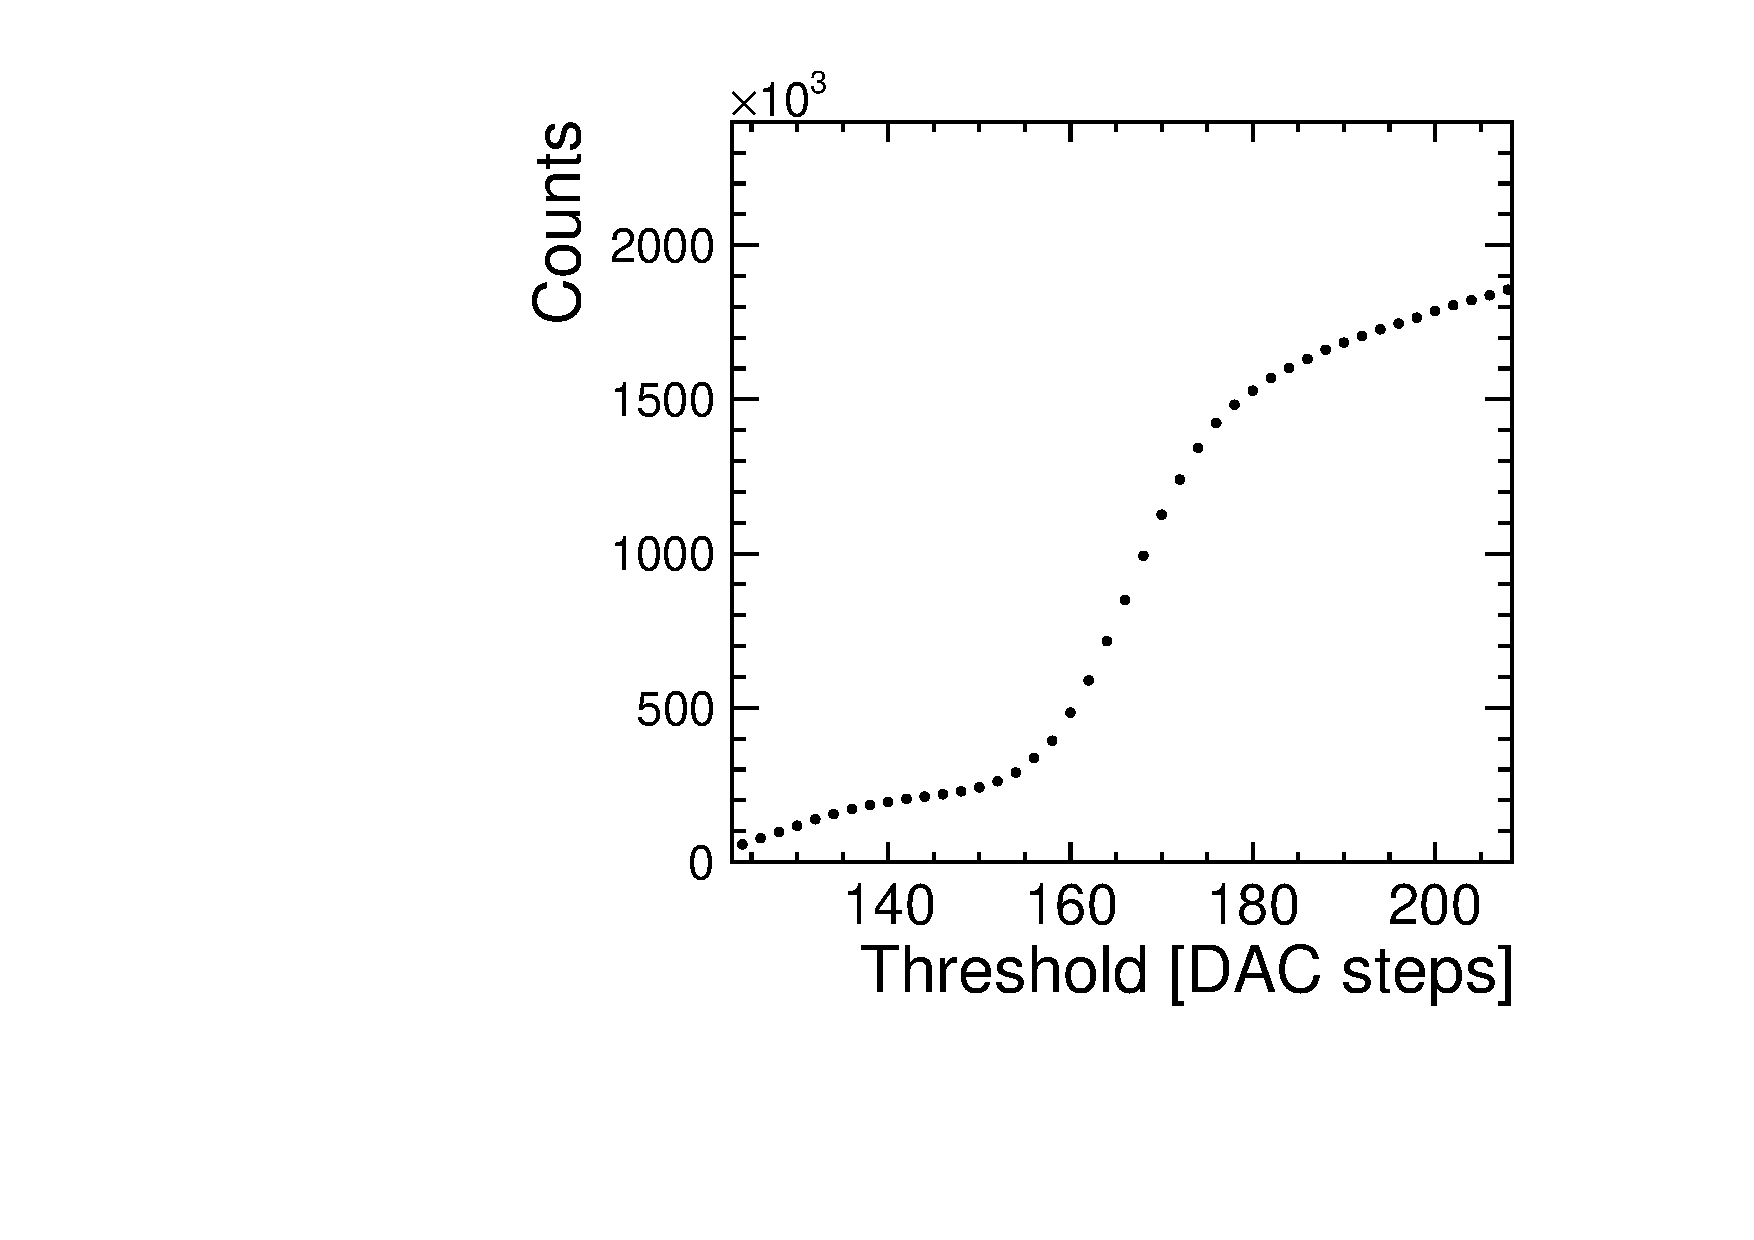
\includegraphics[width=\textwidth]{./figures/Calibration/L04-W0125_scurve_In.pdf}};
    %   % \draw[->,line width=.4pt, color=black](1.8, 1.4) -- (2.4, 1.4);
    %   \node[left, color=black] at (1.9, 1.6) {$K_{\beta}$}; %\draw[->,line
    %   width=.4pt, color=black](3, 2.7) -- (3.7, 2.7); \node[left,
    %   color=black] at (3.5, 2.7) {$K_{\alpha}$};
    % \end{tikzpicture}
    \caption{Measured S-curve}
    \label{fig:scurve_example}
  \end{subfigure} \hfill
  \begin{subfigure}[b]{0.45\textwidth}
    % 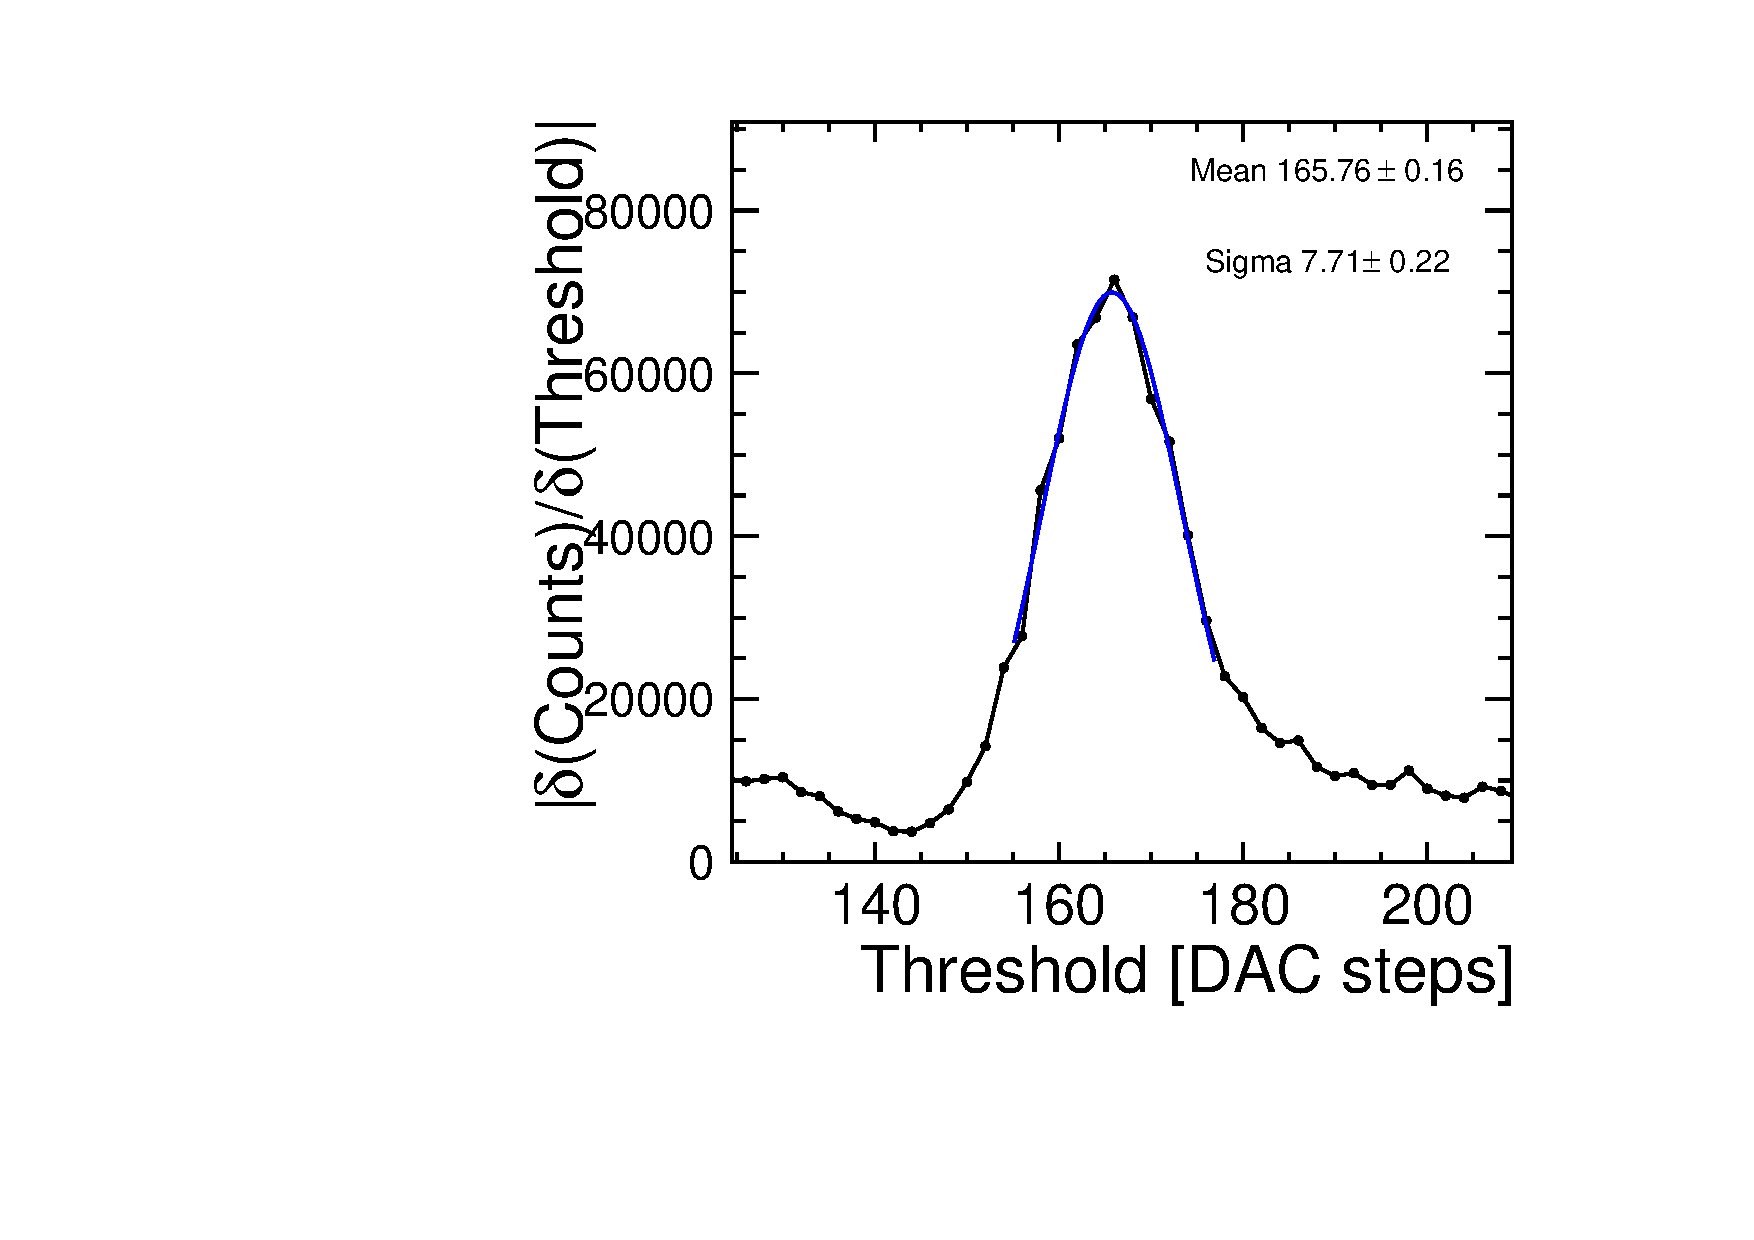
\includegraphics[width=\textwidth]{./figures/Calibration/L04-W0125_scurveDeriv_In.pdf}
    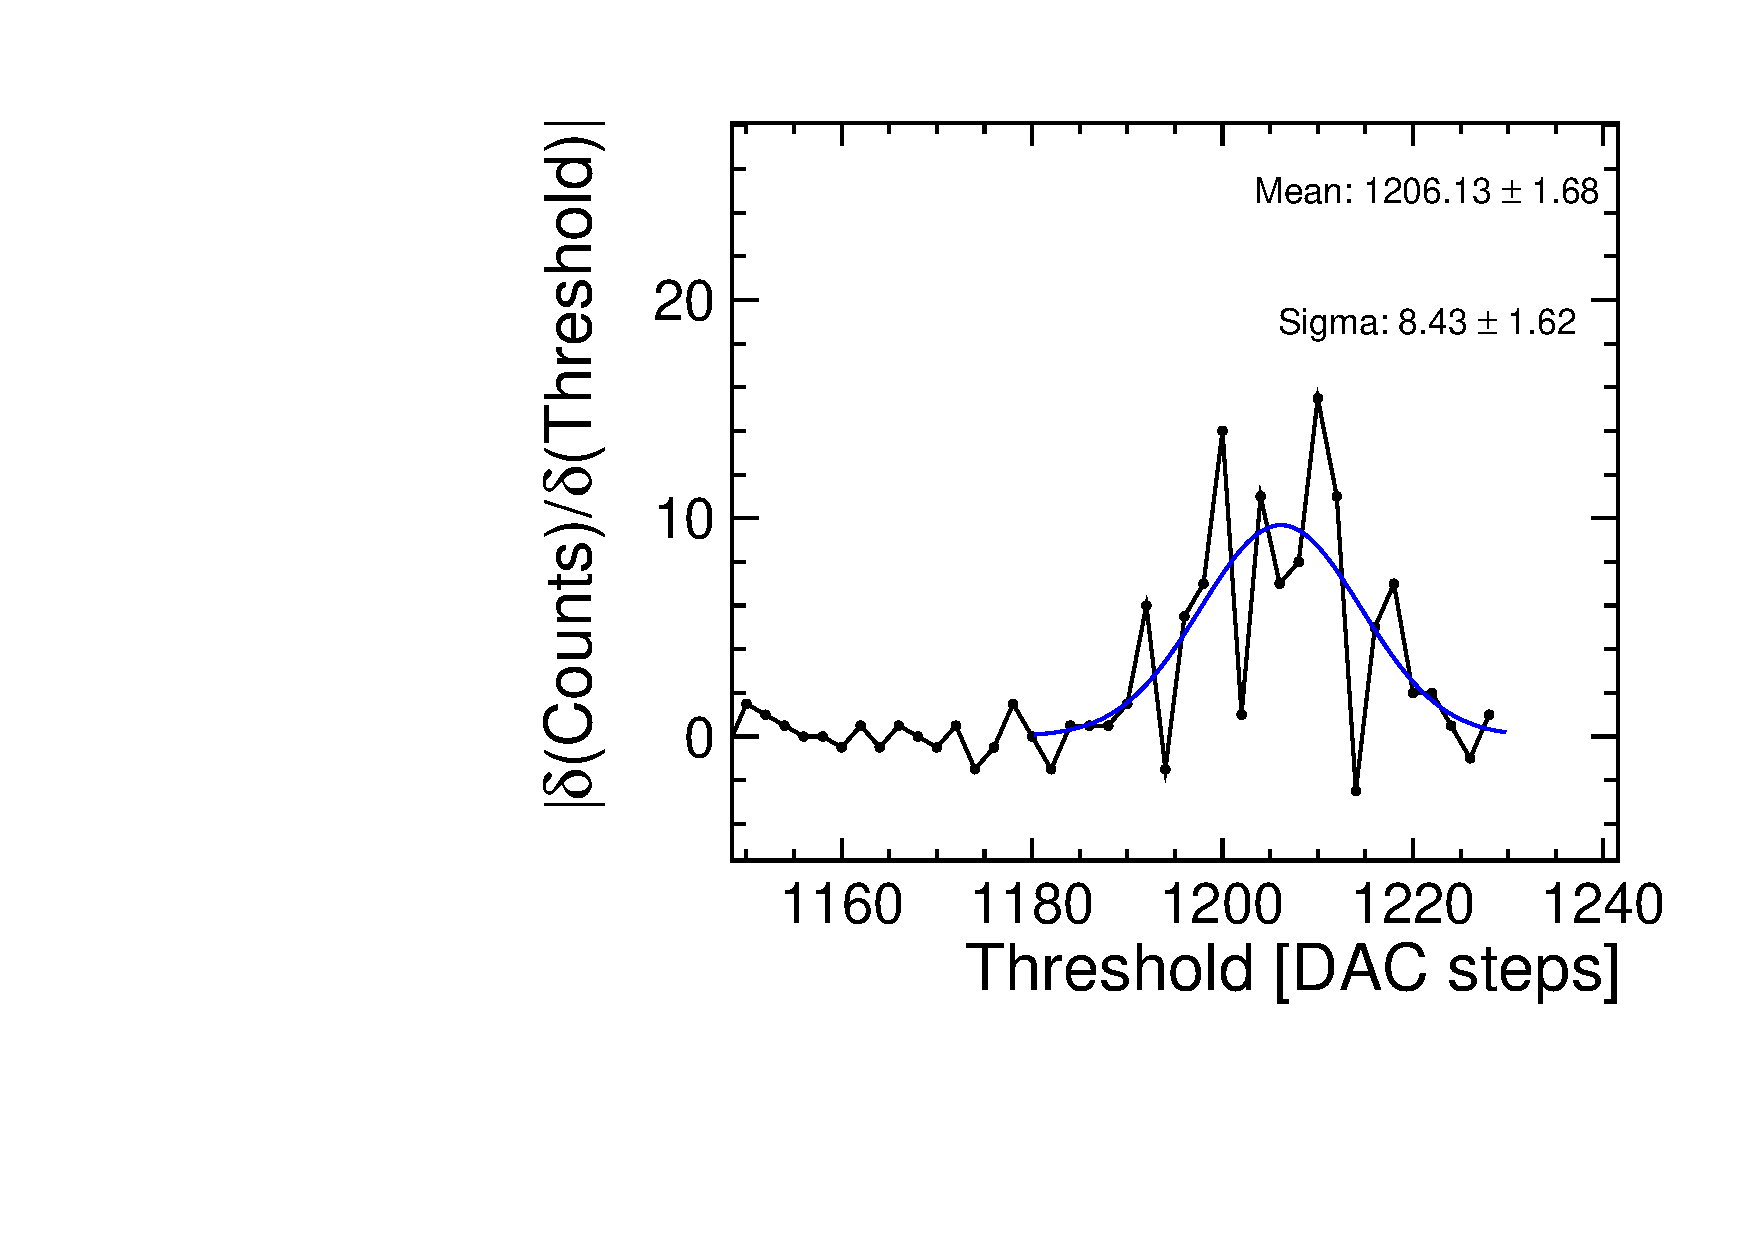
\includegraphics[width=\textwidth]{./figures/Calibration/W5_E2_deriv_scurve_ampl1.pdf}
    \caption{Derivative of the S-curve}
    \label{fig:deriv_example}
  \end{subfigure}
  \caption{An example of a measured S-curve (a) and its derivative
    fitted with a Gaussian function (b) for the assembly W5\_E2 using
    a pulse height of 1000 electrons for the pixel (0, 0). This
    measurement is performed for all the pixels on the diagonal of the
    matrix for each assembly. The threshold DAC is scanned with a step
    size of 2.}
  \label{fig:scurve_deriv_example}
\end{figure}

A linear fit is used to parametrise the relationship between the pulse
height and the threshold DAC given by the mean of the derivative of
the S-curves:
\begin{equation}
  THL_{DAC}=p \; THL_{e-} + q \; ,
  \label{eq:THLDAC}
\end{equation}
where $THL_{DAC}$ is the threshold DAC setting and $THL_{e-}$ the
corresponding energy (in number of electrons). 

\cref{fig:THLcalib_55-GNDGR-100} shows an example of the threshold
calibration obtained for the assembly W5\_E2. Each point used for the
fit corresponds to the mean of the Gaussian fitted to the derivative
of the S-curve for each pulse height. The error on each point
corresponds to the error on the mean of the fitted Gaussians of all
diagonal pixels combined using the propagation of errors.

\begin{figure}[htbp]
  \centering
  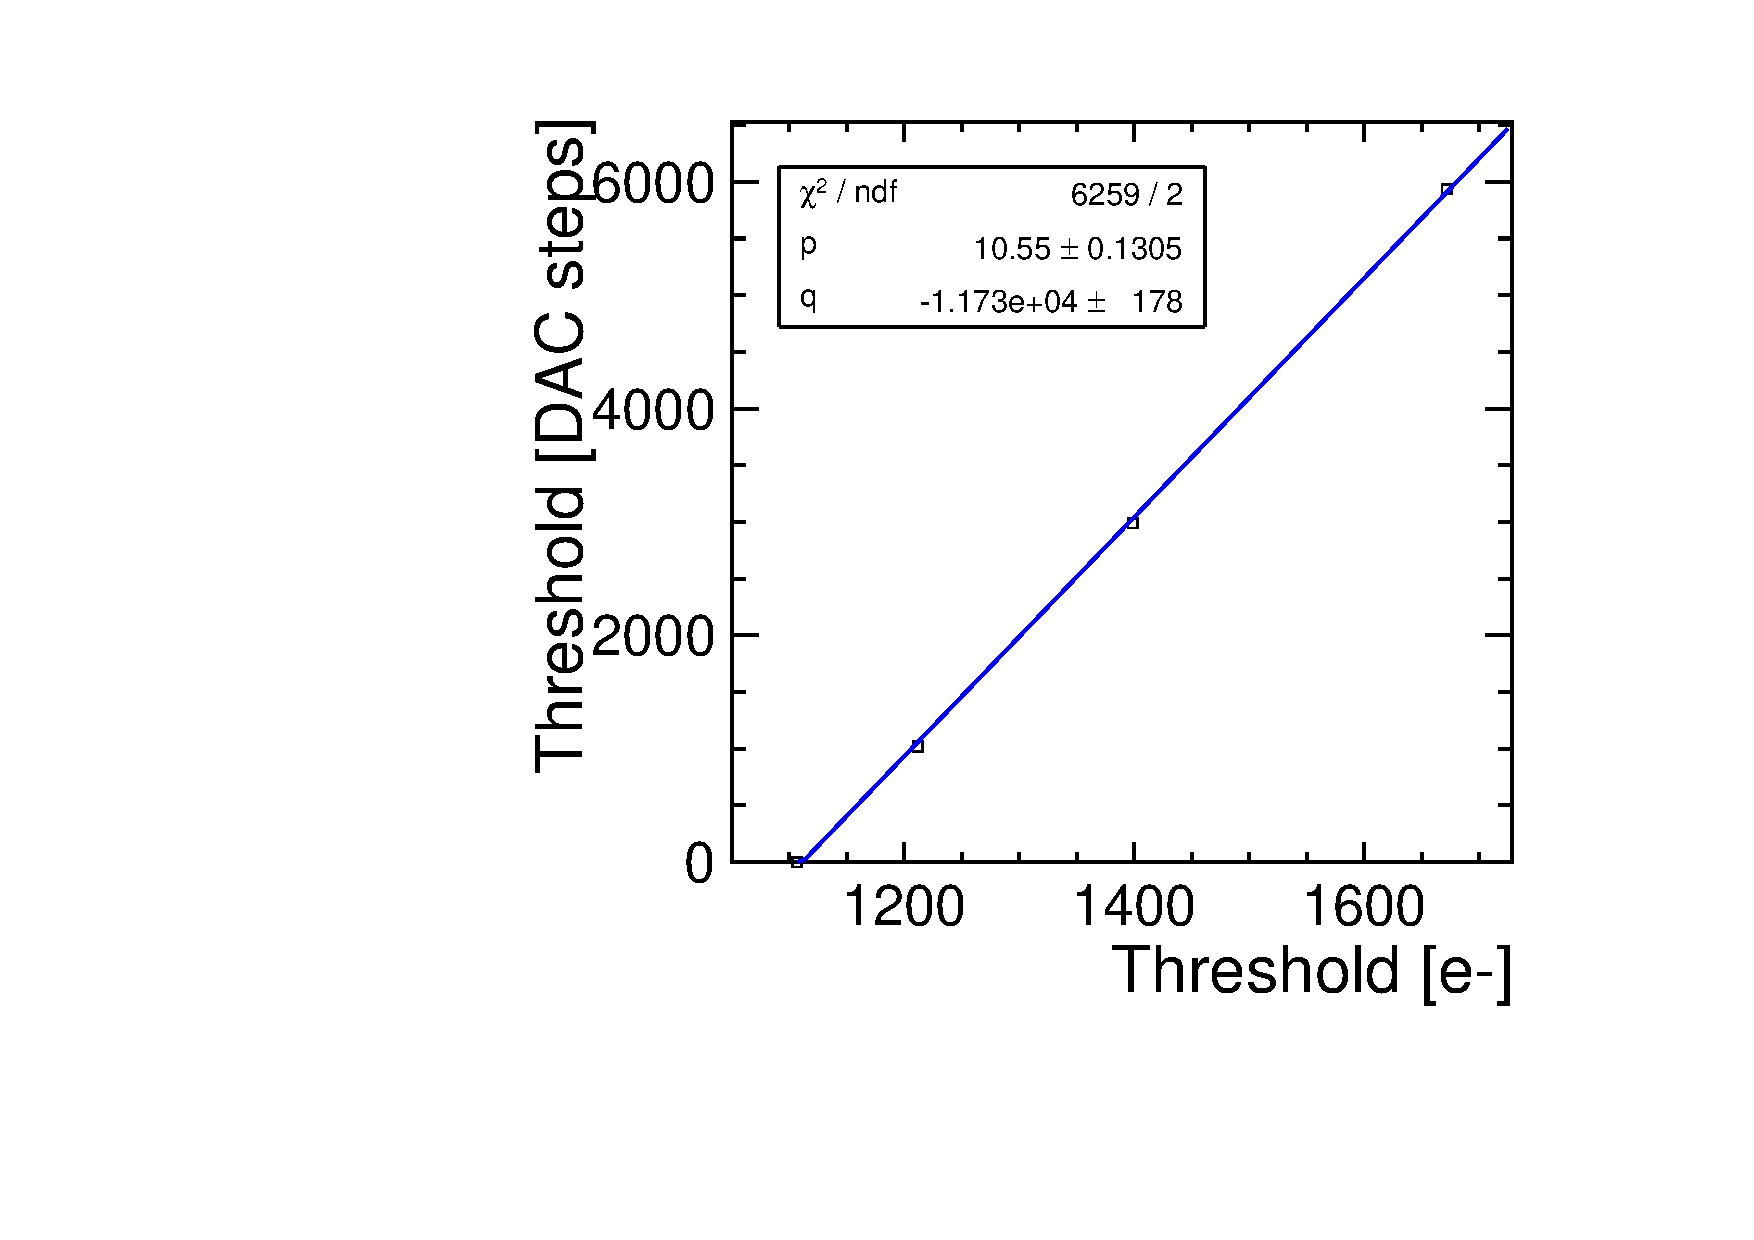
\includegraphics[width=0.5\textwidth]{./figures/Calibration/THLcalibration_W0005_E02.pdf}
  \caption{Threshold calibration for W5\_E2. Each point corresponds to
    the maximum gradient of the S-curve for each pulse height. A
    linear function as described in \cref{eq:THLDAC} was used to fit
    the data points and obtain the parameters $p$ and $q$.}
  \label{fig:THLcalib_55-GNDGR-100}
\end{figure}

% \begin{figure}[htbp]
%   \centering
%   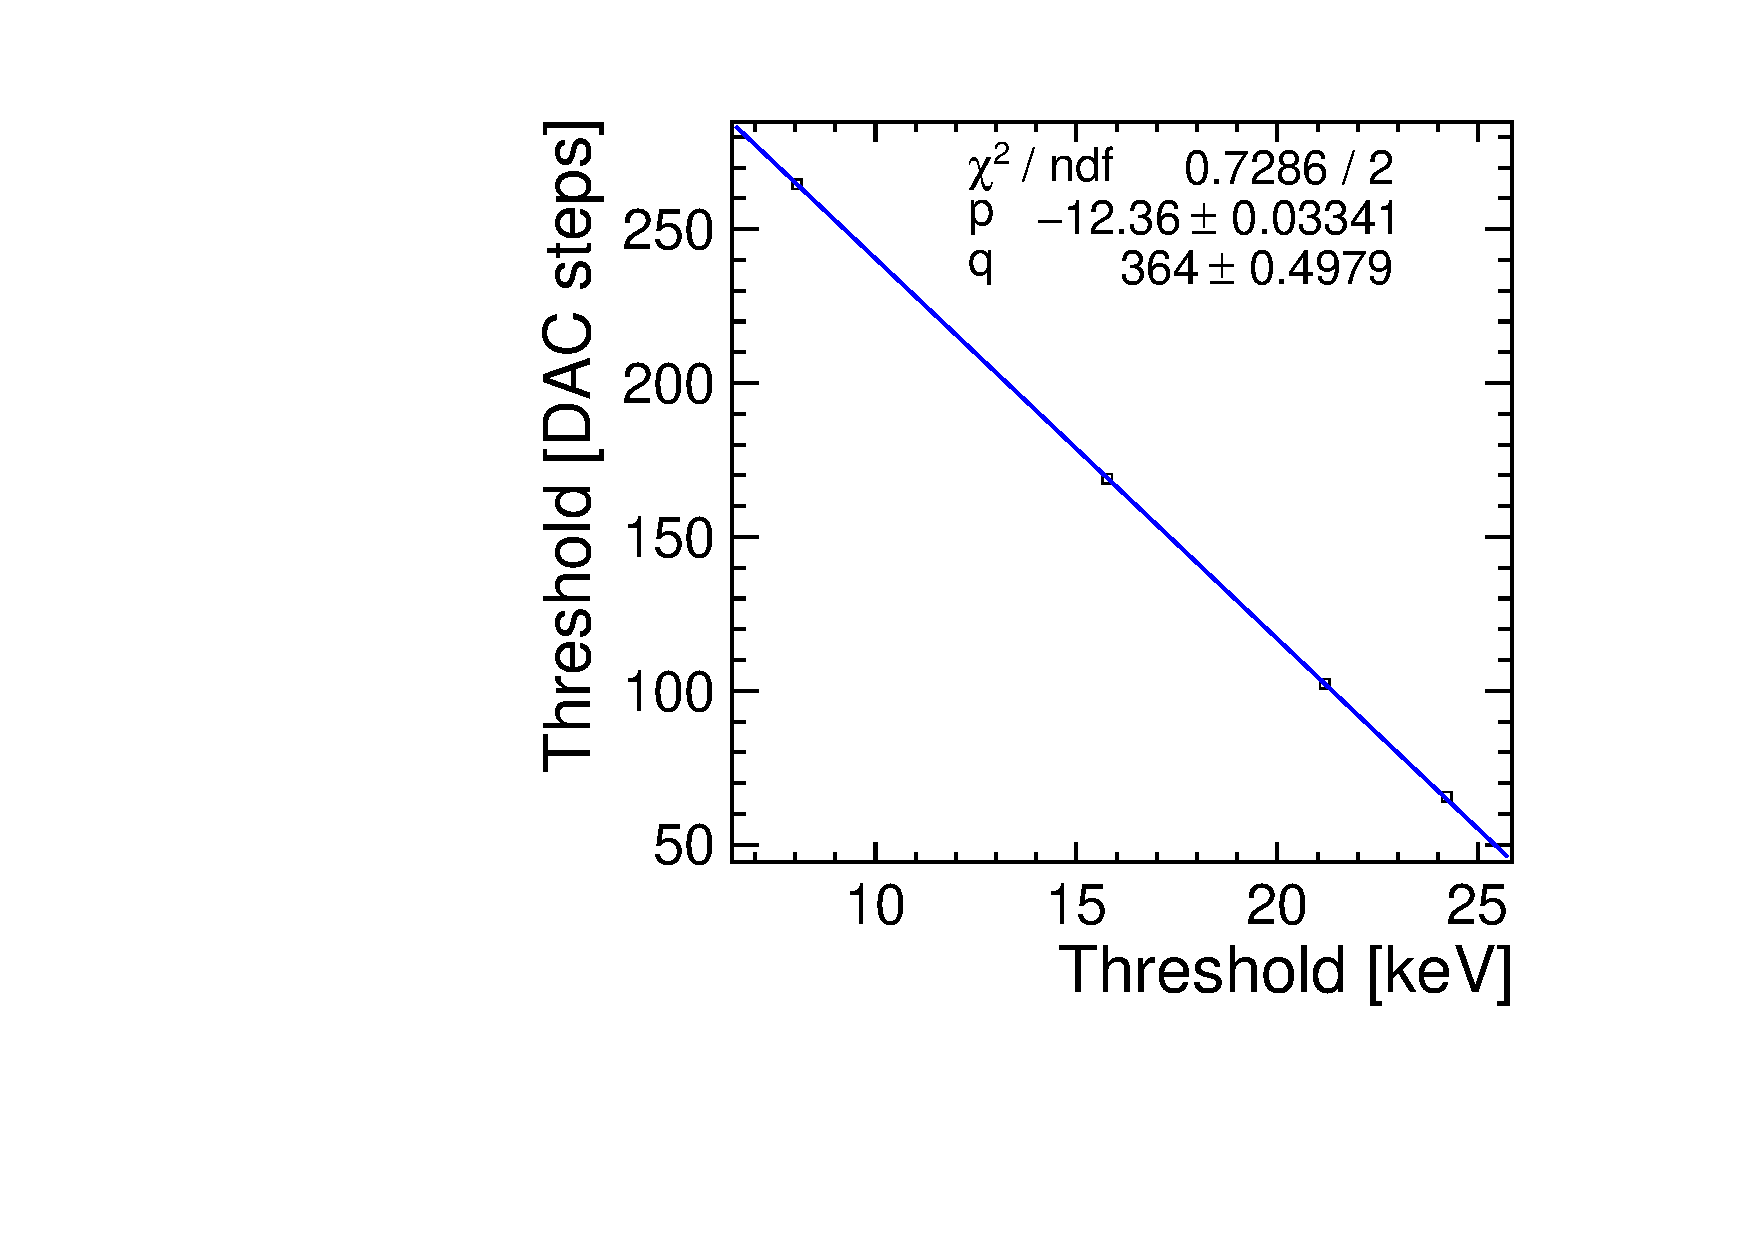
\includegraphics[width=0.5\textwidth]{./figures/Calibration/A06-W0110_THLcalibration.pdf}
%   \caption{Threshold calibration for A06-W0110. Each point corresponds
%     to the maximum gradient of the S-curve for each target (Cu, Zr, Pd
%     and In). A linear function as described in \cref{eq:THLDAC} was
%     used to fit the data points and obtain the parameters $p$ and
%     $q$.}
%   \label{fig:THLcalib_A06}
% \end{figure}

The operating threshold DAC for each assembly was converted to an
energy by solving \cref{eq:THLDAC} for $THL_{e-}$ with
$THL_{DAC}=THL_{DAC}^{op}$. The error on the evaluated threshold in energy
($THL_{e-}^{op}$) is obtained by the propagation of errors for the
inverse of \ref{eq:THLDAC}:
\begin{equation}
  \sigma_{THL_{e-}}^2(THL_{DAC})={{{(THL_{DAC}-q)^2} \over {p^4}} \sigma_{p}^2} +
        {\frac{1}{p^2} \sigma_{q}^2}+
        {2 {{THL_{DAC}-q} \over p^3} \sigma_{pq}^2} \; ,
        \label{eq:THLerror}
\end{equation}
where $p$, $q$ are given by the linear fit using \cref{eq:THLDAC} with
standard deviations $\sigma_{p}$, $\sigma_{q}$ and covariance
$\sigma_{pq}$.

\cref{tab:THLcalibration} summarises the fit parameters p and q, the
operating threshold DAC and its conversion into energy deposition in
number of electrons for all the assemblies listed in
\cref{tab:THLcalibration}.

\begin{table}[htbp]
  \centering
  \caption{Threshold fit parameters p and q, the operating threshold
    DAC and its conversion into energy deposition.}
  \label{tab:THLcalibration}
  \begin{tabular}{lcccc}
    \toprule
    Assembly & p [DAC steps/e\textsuperscript{-}] & q [DAC steps] & THL\textsubscript{DAC}\textsuperscript{op} [DAC steps] & THL\textsubscript{e-}\textsuperscript{op} [e\textsuperscript{-}] \\
    \midrule
    W19\_G7 & $0.087\pm0.000$ & $1144.037\pm0.005$ & 1190 & $526.230\pm0.649$ \\
    W19\_F7 & $0.092\pm0.000$ & $1131.874\pm0.009$ & 1187 & $600.406\pm0.551$ \\
    W19\_L8 & $0.090\pm0.000$ & $1082.057\pm0.005$ & 1133 & $568.506\pm0.538$ \\
    W19\_C7 & $0.091\pm0.000$ & $1092.887\pm0.005$ & 1148 & $608.700\pm0.488$ \\
    W5\_E2 &  $0.095\pm0.000$ & $1106.921\pm0.004$ & 1160 & $561.019\pm0.712$ \\
    W5\_F1 & $0.089\pm0.000$ & $1103.618\pm0.004$ & 1153 & $554.885\pm0.493$ \\
    W2\_J5 & $-0.109\pm0.000$& $1232.643\pm0.034$ & 1170 & $565.723\pm1.560$\\
    \bottomrule
  \end{tabular}
\end{table}



For further verification of these results, the Timepix3 DAC step gain
for each assembly is calculated to be around
11~$\pm$e\textsuperscript{-}/step, in agreement
with~\cite{Timepix3Poikela}. 

Without any test-pulse injection, the threshold scan results in a
Gaussian distribution. The mean of the Gaussian distribution defines
the baseline of the chip and its width, the electronic noise. For all
assemblies the noise varies between 6 to 7 DAC values which
corresponds to 70 to 80 electrons, again in agreement
with~\cite{art:tmpx} (the error is obtained by error propagation of
\cref{eq:THLDAC}). Except for the assembly W2\_J5 which appears to be
noisy. \cref{tab:THLcalibration_noise} summarises the baseline mean,
the threshold DAC step, the electronic noise and its conversion into
energy deposition for the assemblies listed in
\cref{tab:THLcalibration}.


%%%%%%%%%%%%%%%%%%%%%%%%%%%%%%%%%%%%%%%%%%%%%%%%%%

\begin{table}[htbp]
  \centering
  \caption{Measured baseline mean, threshold DAC step gain, the electronic noise
    and its conversion into energy deposition.}
  \label{tab:THLcalibration_noise}
  \resizebox{\textwidth}{!}{\begin{tabular}{lcccc}
    \toprule
    Assembly & Baseline mean [DAC steps] & Threshold DAC step [e\textsuperscript{-}] & Noise [DAC steps] & Noise [e\textsuperscript{-}] \\
    \midrule
    W19\_G7 & $1143.992\pm0.005$ & $11.450\pm0.000$ & $6.864\pm0.005$ & $78.585\pm0.056$ \\
    W19\_F7 & $1131.664\pm0.009$ & $10.892\pm0.000$ & $7.060\pm0.009$ & $76.891\pm0.098$ \\
    W19\_L8 & $1081.998\pm0.005$ & $11.160\pm0.000$ & $6.996\pm0.005$ & $78.078\pm0.058$ \\
    W19\_C7 & $1092.825\pm0.005$ & $11.044\pm0.000$ & $7.413\pm0.005$ & $81.870\pm0.051$ \\
    W5\_E2  & $1106.895\pm0.004$ & $10.570\pm0.000$ & $7.155\pm0.004$ & $75.628\pm0.046$ \\
    W5\_F1  & $1103.591\pm0.004$ & $11.237\pm0.000$ & $6.711\pm0.004$ & $75.408\pm0.046$ \\
    W2\_J5  & $1231.70\pm0.034$ & $-9.177\pm0.000$ & $11.826\pm0.041$ & $108.53\pm0.379$ \\
    \bottomrule
  \end{tabular}}
\end{table}

%%%%%%%%%%%%%%%%%%%%%%%%%%%%%%%%%%%%%%%%%%%%%%%%%%%%%%%%
%%%%%%%%%%%%%%%%%%%%%%%%%%%%%%%%%%%%%%%%%%%%%%%%%%%%%%%%
%%%%%%%%%%%%%%%%%%%%%%%%%%%%%%%%%%%%%%%%%%%%%%%%%%%%%%%%
% \begin{table}[htbp]
%   \caption{Measured DAC step gain.}
%   \label{tab:DACStep}
%   \centering
%   \begin{tabular}{ c c c }
%     \toprule
%     Assembly & Threshold DAC step [\ev] & Threshold DAC step [\Pem] \\
%     \midrule
%     A06-W0110  & $81\pm0.009$ & $22.475\pm0.025$  \\
%     C04-W0110  & $85\pm0.039$ & $23.544\pm0.011$ \\
%     L04-W0125 &  $86\pm0.022$ & $23.775\pm0.006$ \\
%     B06-W0125  & $86\pm0.120$ & $23.978\pm0.033$ \\
%     \bottomrule
%   \end{tabular}
% \end{table}

% Threshold measurements were not completed for assemblies B07-W0125 and
% D09-W0126. Assembly B07-W0125 did not fully deplete due to a broken
% corner of the sensor. The derivative of the CuXRF S-curve did not form
% a peak as the photon energy was close to the noise level. Assembly
% D09-W0126 was not operating as expected for a $100\,\micron$
% sensor. Therefore the calibration of these assemblies was done without
% threshold measurements.



%% \begin{table}[htbp]
%%   \centering
%%   \caption{Advacam active-edge n-in-p planar pixel sensor assemblies. The edge distance is defined by the distance between the last pixel implant and the physical sensor edge.}
%%   \label{tab:NominalThreshold}
%%   \resizebox{\textwidth}{!}{\begin{tabular}{lccc}
%%       \toprule
%%       Assembly & Nominal THL\textsubscript{DAC}\textsuperscript{op} [DAC steps] & Nominal THL\textsubscript{e-}\textsuperscript{op} [electrons]\\
%%       \midrule
%%       20-NGR & 1190 & 466.5\\
%%       23-FGR & 1187 & 532.4\\ \hline
%%       28-GNDGR & 1133 & 517.8\\
%%       55-GNDGR & 1148 & 553.7\\
%%       55-GNDGR-100 & 1160 & 537.9\\ \hline
%%       55-GNDGR-150 & 1153 & 441.2\\
%%       \bottomrule
%%   \end{tabular}}
%% \end{table}


% \begin{table}[htbp]
%   \caption{Threshold fit parameters $p$ and $q$, the operating
%     threshold DAC and its conversion into energy.}
%   \label{tab:evalTHL} 
%   \centering
%   \begin{tabular}{ c c c c c }
%     \toprule
%     Assembly & $p$ [DAC steps/\kev] & $q$ [DAC steps] & $THL_{DAC}^{op}$ [DAC steps] & $THL_{\kev}^{op}$ [\kev] \\
%     \midrule
%     A06-W0110 & $-12.36\pm0.03$ & $364.0\pm0.50$ & 326 & $3.077\pm0.033$ \\
%     C04-W0110 & $-11.8\pm0.02$ & $441.6\pm0.42$ & 405 & $3.102\pm0.030$ \\
%     L04-W0125 & $-11.68\pm0.02$ & $448.6\pm0.31$ & 410 & $3.303\pm0.023$ \\
%     B06-W0125 & $11.58\pm0.037$ & $390.6\pm0.80$ & 435 & $3.836\pm0.057$ \\
%     \bottomrule
%   \end{tabular}
% \end{table}
